% !Mode:: "TeX:UTF-8"

%软件层面还需要加上补偿(包括回滚),表重画为三线表;缺业务层面不确定性建模(A*),重画状态动作关系表;

\section{目前已完成的研究工作及结果}

本课题分为4个部分,它们之间的关系如图所示。已经完成的工作内容包括(1)-(4)部分的服务不确定性建模、基于基于价值的软件层服务不确定性决策、基于基于价值的业务层服务不确定性决策以及支持不确定性决策的仿真系统。其中(1)不确定性建模和(4)支持不确定性决策的仿真系统已经完成,(2)基于价值的软件层服务不确定性决策和(3)基于价值的业务层服务不确定性决策也已经完成,但尚需更多和更具体的测试程序进行算法的有效性和复杂性进行测试。

\subsection{服务不确定性建模} \label{sec:model_section}

本部分在硕士论文的开题之前已经完成大部分内容,以下作简要介绍。

针对软件层服务,需要对服务方案、不确定性事件、服务执行的状态进行建模,同时本课题提出不确定性事件触发关系图~(UTG)~并对此进行建模。
%为了度量决策的优劣,需要对决策收益(价值)进行建模。

\subsubsection{服务方案}

使用服务流程表示当前执行中的服务方案,表示为如式(\ref{equation:splan})所示。
\begin{equation}\label{equation:splan}
SPlan = \left( {A,E,fc,dc} \right)
\end{equation}
\begin{tabularx}{\textwidth}{@{}l@{\quad}l@{\pozhehao }X@{}}
    式中
    & ${A}$ & 活动集合,表示为~$\{{a_1}, {a_2},...,{a_n}\}$ ~; \\
    & ${E}$ & 活动之间的时序依赖关系,表示为~$\{{e_1}, {e_2},...,{e_n}\}$ ~;\\
    & ${fc}$ & 服务若执行失败,提供方需要支付给客户的补偿金;\\
    & ${dc}$ & 表示服务若执行延期,每单位时间延迟需要支付给客户的补偿金。
\end{tabularx}\vspace{\wordsep}

针对每个活动,可表示为如如式(\ref{equation:activity})所示。
\begin{equation}\label{equation:activity}
{a_i} = ({CS_i}, {S_{i0}}, {LST_i}, {LET_i})
\end{equation}
\begin{tabularx}{\textwidth}{@{}l@{\quad}l@{\pozhehao }X@{}}
    式中
    & ${CS_i}$ & 活动的可替换服务集;\\
    & ${S_{i0}}$ & 当前被选中用于执行该活动$i$的具体服务;\\
    & ${LST_i}$ & 最晚开始时间;\\
    & ${LET_i}$ & 最晚结束时间;
\end{tabularx}\vspace{\wordsep}

针对活动之间的依赖关系,一般的服务流程中存在各种复杂结构关系,本文考虑串行与并行两种关系,并使用如式(\ref{equation:e})表示,其意义是活动${a_j}$需要在活动${a_i}$执行完成后才能开始执行,在~DAG~图中体现的则是从结点${a_i}$到结点${a_j}$之间有一条有向边。
\begin{equation}\label{equation:e}
e = ({a_i},{a_j})
\end{equation}

对于候选服务,是以服务编号和~QoS~组成的二元组,如式(\ref{equation:cs})所示。其QoS是以执行时间~$t$~、价格~$p$~,可靠性~$r$~组成的三元组,如式(\ref{equation:qos})所示。

\begin{equation}\label{equation:cs}
CS = (id, QoS)
\end{equation}

\begin{equation}\label{equation:qos}
QoS = (t, p, r)
\end{equation}

\subsubsection{软件层不确定性建模}
本课题关注的是服务执行过程中从外界可观测到的事件,即站在服务使用者的角度观察系统的运行状态,而不关心服务执行环境内部是何种原因而产生的事件。这样做的原因是服务方案通常是由服务中介方负责构建的,方案中使用的各服务并不受其控制,故只能从外部观察。

事件可表示为如式(\ref{equation:event})所示,其中t为事件发生的时刻,a为事件所涉及的活动,EType表示事件的类型。
\begin{equation}\label{equation:event}
event = (t, a, EType)
\end{equation}
\begin{tabularx}{\textwidth}{@{}l@{\quad}l@{\pozhehao }X@{}}
    式中
    & $t$ & 事件发生的时刻;\\
    & $a$ & 事件所涉及的活动;\\
    & $Type$ &事件的类型。
\end{tabularx}\vspace{\wordsep}

考虑事件的类型~$EType$~。服务执行过程中的产生的事件分为两大类:正常事件、不确定性事件。前者是一项活动按计划正常开始和正常执行结束时所发出,后者是指活动未按预期开始或结束,或者执行失败。按照事件触发的机制,可分为以下三类:

\begin{itemize}
    \item 由定时器所触发的事件,表示某活动未在期望时间点上开始执行或执行完成。服务执行引擎根据服务方案中为每个活动预设的最晚开始和最晚结束时刻对服务执行进行监控,如果到达~$LST_i$~或~$LET_i$~时刻活动未能开始或结束,将发出以下两类事件:
    
    $E_{01}$:~活动~$a_i$~在当前时刻~$t$~未开始执行,满足~$t>LST_i+\delta$~ (~$\delta$~是一个足够小的时间间隔),一旦系统在~$LST_i+\delta$~时刻未发现~$a_i$~开始执行,则发出该类事件;
    
    $E_{02}$:~与之类似,活动~$a_i$~在当前时刻~$t$~未按计划执行结束,满足~$t>LETi+\delta$~;
    
    \item 由活动的开始执行所触发的事件。一旦服务活动开始执行,系统即产生该类事件。
    
    $E_{11}$:~活动准时/提前开始,此时~$t\le LST_i$~。
    
    $E_{12}$:~活动延迟开始,此时~$t>LST_i$~。
    
    \item 由活动执行结束所触发的事件,可分为以下两种情况:
    
    $E_{21}$:~活动执行失败或错误,未得到期望结果;
    
    $E_{22}$:~活动执行成功。~$t\le LET_i$~表示活动提前或准时执行结束,而~$t>LETi$~表示活动有延迟。
    
\end{itemize}

\subsubsection{业务层不确定性建模}

针对业务层服务,与软件层服务有较大区别,因此业务层服务不确定性建模将有别于软件层服务建模。业务层面服务不确定性包括软件层面的服务不确定性,因此,在业务层面执行服务时若出现软件层服务不确定性,可转化为软件层的服务不确定性决策。同时,业务服务有软件服务不具备的特有性质,站在中间人的角度,从用户需求和服务资源两个方面建立业务层服务不确定性模型。

需求和资源的分配如图~\ref{figure:user_resource}~所示,左边是一系列资源,右边为多个用户,发生不确定性之前,资源以及存在一个分配,满足所有用户的需求,服务提供者期望在服务执行结束后获得一定的收益。若发生不确定性,则需求可能不被满足,服务提供者也无法获得收益,这即是在业务层服务不确定性需要解决的问题。

\begin{figure}[htbp]
    \centering
    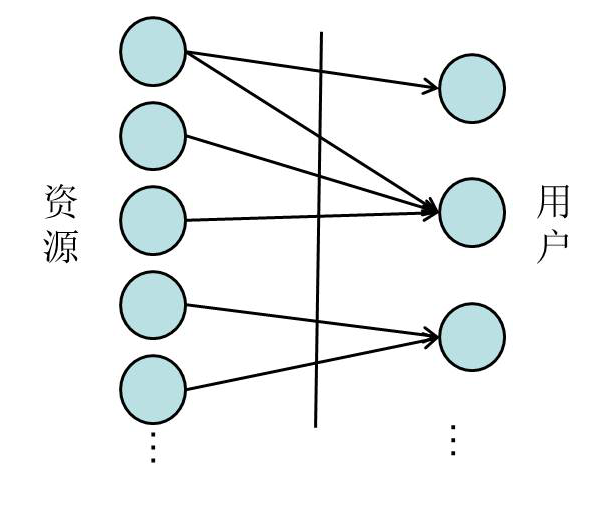
\includegraphics[width = 0.3\textwidth]{user_resource}
    \caption{用户资源的分配}\label{figure:user_resource}
    \vspace{-1em}
\end{figure}

形式化地,资源可表示为如式(\ref{equation:resource})所示的一个向量,向量的每一个维度表示资源的类型。

\begin{equation}\label{equation:resource}
s = (s_1, s_2, ..., s_n)
\end{equation}
\begin{tabularx}{\textwidth}{@{}l@{\quad}l@{\pozhehao }X@{}}
    式中
    & $s_i$ & 第~$i$~个类型的资源。
\end{tabularx}\vspace{\wordsep}

%一个用户的需求可以看作多这多个资源的需求,即可表示为如式(\ref{equation:demand})所示的一个向量。
%\begin{equation}\label{equation:demand}
%w = (w_1, w_2, ..., w_n)
%\end{equation}
%\begin{tabularx}{\textwidth}{@{}l@{\quad}l@{\pozhehao }X@{}}
%    式中
%    & $w_i$ & 对第~$i$~个类型的资源需求重要程度,满足$\sum\limits_{i = 1}^n {{w_i}}  = 1$
%\end{tabularx}\vspace{\wordsep}
%
%则用户对资源的总体需求需要满足的条件如式(\ref{equation:demand_total})所示。
%\begin{equation}\label{equation:demand_total}
%\sum\limits_{i = 1}^n {{w_i}{s_i}}  \ge D
%\end{equation}
%\begin{tabularx}{\textwidth}{@{}l@{\quad}l@{\pozhehao }X@{}}
%    式中
%    & $D$ & 用户对资源的总需求数量。
%\end{tabularx}\vspace{\wordsep}

针对多用户多需求的情况,资源分配则可表示为一个矩阵,如式(\ref{equation:resource_arr})所示,其中行维度是一个用户需求,列维度为资源种类。

\begin{equation}\label{equation:resource_arr}
S = \begin{array}{*{20}{c}}
{{s_{11}}}&{{s_{12}}}& \cdots &{{s_{1n}}}\\
{{s_{21}}}&{{s_{22}}}& \cdots &{{s_{2n}}}\\
\vdots & \vdots & \ddots & \vdots \\
{{s_{m1}}}&{{s_{m2}}}& \cdots &{{s_{mn}}}
\end{array}
\end{equation}
\begin{tabularx}{\textwidth}{@{}l@{\quad}l@{\pozhehao }X@{}}
    式中
    & $s_{ij}$ & 用户~$i$~分配资源~$j$~的数量。
\end{tabularx}\vspace{\wordsep}

很显然,式(\ref{equation:resource_arr})的一列之和为每个类型资源总数,一行中按用户需求比重加权求和为分配到一个用户上的资源总数。

\setcounter{paragraph}{0}
\paragraph{用户需求不确定性描述}

用户在使用服务的过程中,需求难免会发生变化。例如,海运物流中,用户可能发生增加(减少、取消)货物舱位的需求,此时发生的不确定性,船公司需要作出决策,使得既能满足用户需求又能使得自己的收益最大化(或减少得最少)。

形式化地,不确定性事件表示为如式(\ref{equation:demand_event})所示。其中当~$j=0$~时表示用户不关心什么类型的资源增加/减少,只关心资源总量的增加/减少。
\begin{equation}\label{equation:demand_event}
demand\_event = (i, j, \pm n)
\end{equation}
\begin{tabularx}{\textwidth}{@{}l@{\quad}l@{\pozhehao }X@{}}
    式中
    & $i$ & 第$i$个用户,取值范围$1 \cdots n$;\\
    & $j$ & 第$j$个类型的资源,取值范围$0 \cdots n$;\\
    & $\pm n$ & 数量增加/减少$n$;
\end{tabularx}\vspace{\wordsep}

\paragraph{服务资源不确定性描述}

资源同样也会发生变化,例如集装箱损坏了导致集装箱数量减少,或者陆运过程中其中部分车辆临时损坏导致于无法继续运货,体现在如式(\ref{equation:resource})所示中各个变量都可能发生变化。形式化地,定义为如式(\ref{equation:resource_event})所示。

\begin{equation}\label{equation:resource_event}
resource\_event = (j, \pm n)
\end{equation}
\begin{tabularx}{\textwidth}{@{}l@{\quad}l@{\pozhehao }X@{}}
    式中
    & $j$ & 第$j$类资源,取值范围$1 \cdots n$;\\
    & $\pm n$ & 数量增加/减少$n$;
\end{tabularx}\vspace{\wordsep}

需要注意的是,用户的需求发生变化一般发生在服务执行之前,而资源的变化可能发生在执行过程中,也可能发生在服务执行之前。
%
%根据以上三点介绍,可以形式化的表达需要解决的问题。
%
%问题的输入:当前的资源分配方案、不确定性事件列表
%
%问题的输出:资源重新分配方案
%
%优化目标:最大化服务提供者的收益,最小化用户提供的成本。
%
%形式化地,问题表示为...



\subsection{基于价值的软件层服务不确定性决策}

面向不确定性的优化决策的目标可表述为:以最小的时间延迟和成本溢出,使服务可最大概率的进入到“成功结束”状态。

在软件服务环境中,针对服务运行时可能发生的不确定性(风险)进行监听,从而发现故障并采取相应的动作使得服务能够最大限度地正常执行。因此,在\ref{sec:model_section}节介绍的基于价值的服务不确定性建模的基础上,针对软件服务层面对事件、决策和状态之间以及它们之间的关系进行建模,最后基于~MDP~对软件服务不确定性进行求解优化。

\subsubsection{服务执行的状态} 

服务流程在执行过程中产生各种正常或不确定事件,导致服务执行不确定状态。本节给出服务执行状态的刻画。

首先定义活动的状态。对某活动~$a_i$~,其状态可表示为如式(\ref{equation:state})所示。

\begin{equation}\label{equation:state}
state=(a, STATE\_TYPE^{N/U})
\end{equation}
\begin{tabularx}{\textwidth}{@{}l@{\quad}l@{\pozhehao }X@{}}
    式中
    & $T$ & 处于当前状态时相比于预期服务方案的时间延迟~(TimeDelay)~;\\
    & $C$ & 处于当前状态时相比于预期服务方案的成本溢出~(CostOverflow)~;\\
    & $N$ & 该状态为正常状态~(Normal)~,即时间和成本未超出初始服务方案中对~$a_i$~的时间与成本的规划~$(T\le 0, C\le 0)$~;\\
    & $U$ & 该状态为不正常状态~(Uncertain)~,即当前存在时间延迟或者成本溢出~$(T>0, C>0)$~;
\end{tabularx}\vspace{\wordsep}

~$STATE\_TYPE$~可为以下6种类型之一,对~$NOT\_READY$~、~$FAIL$~、~$CANCEL$~三类状态来说,不存在正常或不正常的分类,可不需标注上标~$N$~或~$U$~。

\begin{itemize}
    
    \item ~($NOT\_READY$):~$a_i$~至少有一个前序活动尚未执行结束,故~$a_i$~尚无开始执行的条件,即~$\exists a' \in \{ {a_j}|\exists e = ( {{a_j},{a_i}} )\} ,state ( {a'} ) \ne FINISH \Rightarrow state ( {{a_i}} ) = NOT\_READY$~。这是所有活动的缺省状态。
    
    \item 待执行($READY$):~若~$a_i$~的所有前序活动均已执行完毕(处于~$FINISH$~状态),且对这些活动的决策动作均非“终止”时,ai具备了执行的先决条件,进入该状态,即~$\forall a' \in \{ {a_j}|\exists e = ( {{a_j},{a_i}} )\} ,state ( {a'} ) = FINISH \wedge Action(a') \ne STOP \Rightarrow state ( {{a_i}} ) = READY$~。当~$a_i$~处于READY状态且产生~$E_{01}$~时,它仍然处于~$READY$~状态;
    
    \item 执行中($EXEC$):~当本活动产生~$E_{11}$~、~$E_{02}$~事件时,~$a_i$~正在执行中,但尚未结束;
    
    \item 执行后失败($FAIL$):~本活动产生~$E_{21}$~事件,~$a_i$~执行结束,但未得到期望输出,执行失败;
    
    \item 执行后成功~($FINISH$):~本活动产生~$E_{22}$~事件,~$a_i$~执行结束,已得到期望结果;
    
    \item 取消~($CANCEL$):~当某活动处于~$READYU$~、~$FINISHU$~或~$FAIL$~状态,并且决策动作将该活动终止时,~$a_i$~被人为取消,服务方案停止执行而完全失败。
\end{itemize}

%事件或决策动作导致活动的状态变化。
状态之间的转换关系如图~\ref{figure:state_trans}~所示。
\begin{figure}[htbp]
    \centering
    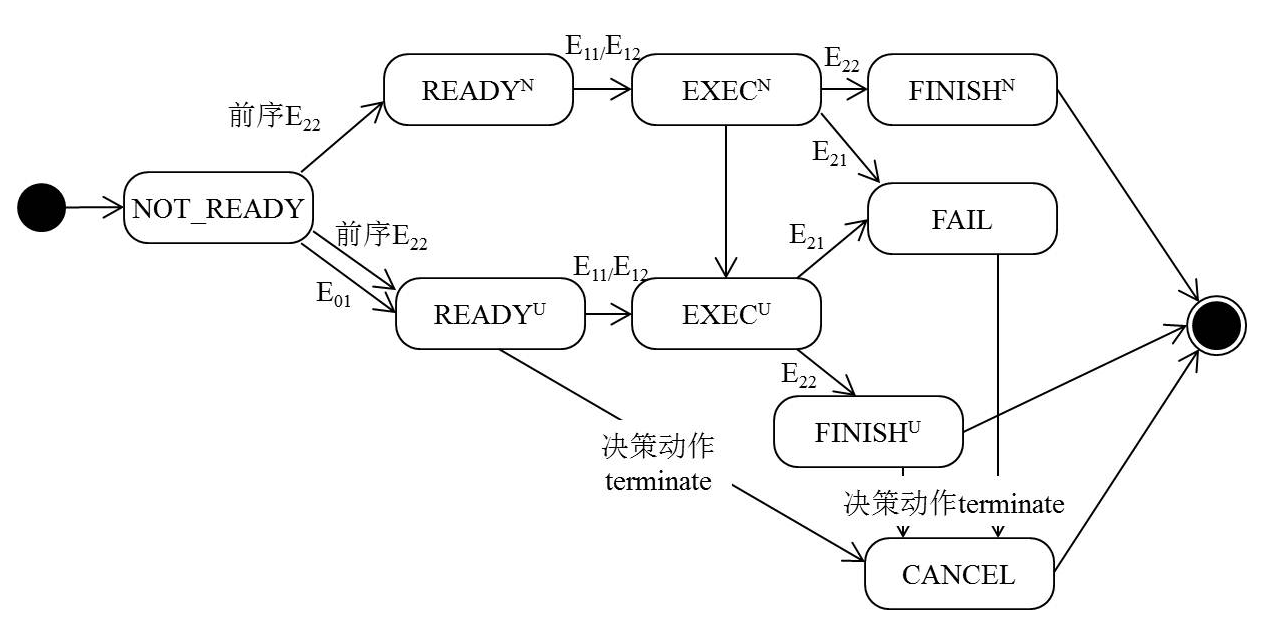
\includegraphics[width = 0.6\textwidth]{state_trans}
    \caption{服务活动的状态转换关系}\label{figure:state_trans}
    \vspace{-1em}
\end{figure}

%(2) 服务执行的整体状态
%
%将服务执行“前锋线”~(forward line)~上的各服务活动的状态联合起来,共同表示服务执行的整体状态~state(SPlan)~,如式(\ref{equation:state_total})所示。
%
%\begin{equation}\label{equation:state_total}
%state = < state(a_i),state(a_{i+1}),..., state(a_j)>
%\end{equation}
%\begin{tabularx}{\textwidth}{@{}l@{\quad}l@{\pozhehao }X@{}}
%    式中
%    & $state(a_i)$ & 活动~$a_i$~的状态。
%\end{tabularx}\vspace{\wordsep}
%
%所谓的“前锋线”~(Front Line)~,是指将已经执行的部分和尚未执行的部分分开的一条线,表示为~$FL(SPlan)=\{(a_i, state(a_i))\}$~,它由一组活动及其状态构成,~$prodecessor(FL)$~、~$successor(FL)$~分别为其左侧和右侧的活动集合。处于~$FL$~中的每一个服务,可能是~$READY^{N/U}$~、~$EXEC^{N/U}$~、~$FAIL$~、~$FINISH^{N/U}$~的某一状态,其所有前序活动的状态必须是~$FINISH^{N/U}$~,其所有后序活动的状态必须是~$NOT\_READY$~,即
%$\forall {a_i} \in FL,state({a_i}) \in \{ READ{Y^{N/U}},{\rm{ }}EXE{C^{N/U}},{\rm{ }}FAIL,{\rm{ }}FINIS{H^{N/U}}\} ;\forall a' \in predecessor(FL),state(a') = FINIS{H^{N/U}};\forall a' \in successor(FL),state(a') = NOT\_READY.$
%
%例如,在某一时刻服务执行状态如图~\ref{figure:front_line}~所示,虚线表示流程执行的前锋线,它左侧的活动~$(a_1, a_2, a_5)$~均处于~$FINISH$~状态,它右侧的活动~$(a_7, a_8, a_9)$~均处于~$NOT\_READY$~状态,而在线上的三个活动~$(a_3, a_4, a_6)$~,分别处于~$READY$~、~$EXEC$~、~$FAIL$~状态。
%
%\begin{figure}[htbp]
%    \centering
%    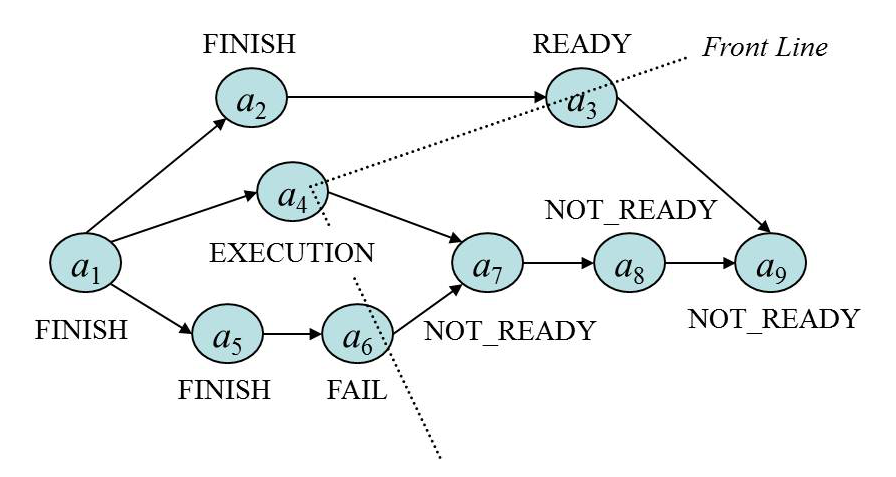
\includegraphics[width = 0.5\textwidth]{front_line}
%    \caption{服务方案执行中的状态划分与前锋线}\label{figure:front_line}
%    \vspace{-1em}
%\end{figure}
%
%%~$state(SPlan)$~可分为几类:
%\begin{itemize}
%    \item 执行前: ~$predecessor(FL) = \emptyset ,$ 对 $ \forall {a_i} \in FL,state({a_i}) = READ{Y^N}$~;
%    \item 执行中: ~$FL \ne \emptyset ,predecessor(FL) \ne \emptyset ,successor(FL) \ne \emptyset $~;
%    \item 执行结束(成功): ~$FL = \emptyset ,successor(FL) = \emptyset ,$ 对 $\forall {a_i} \in predecessor(FL),state({a_i}) = FINIS{H^{N/U}}$~;
%    \item 执行结束(失败): ~$FL \ne \emptyset ,$ 且 $\exists {a_i} \in FL,state({a_i}) = FAIL$~;
%\end{itemize}

%\subsubsection{不确定性触发关系图~(UTG)~} 
%不确定性本身蕴含着服务的一种状态(不正常状态),它是可以传播的,若不采取任何对策(不作为),任由某一不确定性蔓延下去,将会造成更严重的后果(成本溢出、时间延误、执行失败)。即使采取了某一种对策,弥补了某些潜在后果,但可能不会完全弥补,因此也会扩散。这里提出不确定性触发关系图~(Uncertainty Triggering Graph, UTG)~表达~UC~之间的触发关系。利用~UTG~来计算不确定性事件及决策动作所引发的直接和间接代价。
%
%UTG可表示为包含两类节点和两类边的有向图~UTG = ~$(rs, SS, AS, TSA, TAS)$,其中:
%\begin{itemize}
%    \item ~$rs=(a_i, state_i)$~表示根状态,代表活动~$a_i$~处于~$state_i$~时所生成的UTG;
%    \item ~$SS={ss}$~为状态节点集合,其中包含两类节点:第一类为原子状态~$ss=(a_j, state_j)$~,第二类为嵌套的~UTG~根结点,可扩展为一棵完整的~UTG~树;
%    \item ~$AS={action}$~为决策动作节点的集合;
%    \item ~$TSA=ss \to action$~表示状态节点到决策动作节点的有向边;
%    \item ~$TAS=action \to ss$~表示决策动作节点到状态节点的有向边,它具有三个属性:~$tp$~(该状态转移的概率)、~$\Delta T$~(该状态转移所造成的时间延迟)、~$\Delta C$~(该状态转移所造成的成本增加)。
%\end{itemize}
%
%如图~\ref{figure:utg_tree}~给出了~UTG~示意图,其中菱形框表示根状态,圆形节点表示原子状态,矩形框表示决策动作节点,箭头表示~$TSA$~和~$TAS$~。
%
%\begin{figure}[htbp]
%    \centering
%    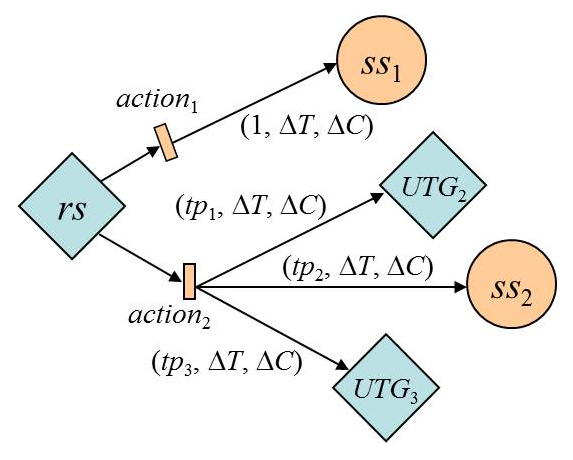
\includegraphics[width = 0.3\textwidth]{utg_tree}
%    \caption{不确定性事件触发关系图~(UTG)~}\label{figure:utg_tree}
%    \vspace{-1em}
%\end{figure}
%
%在~UTG~模型中,状态节点可以是一棵~UTG~的根节点,这代表了不同~UTG~之间的连接(不同活动的不确定性状态之间的转换)。若将此类~UTG~节点展开,即可形成如图~\ref{figure:many_utg_tree}~所示的形态。
%
%\begin{figure}[htbp]
%    \centering
%    \includegraphics[width = 0.5\textwidth]{many_utg_tree}
%    \caption{多棵UTG的连接~(UTG)~}\label{figure:many_utg_tree}
%    \vspace{-1em}
%\end{figure}
%
%如图~\ref{figure:utg_example}~给出一个小例子。假设服务方案是由三个活动~$(a_1, a_2, a_3)$~串行构成的流程,图~(a)~表示活动~$a_1$~在~$READY^U$~状态下的~UTG~,~(b)~表示活动~$a_1$~在~$FINISH^U$~状态下的~UTG~,~(c)~表示~$a_1$~在~$FAIL$~状态下的~UTG~。
%
%\begin{figure}[htbp]
%    \centering
%    \includegraphics[width = 0.5\textwidth]{utg_example}
%    \caption{~UTG~的三个例子}\label{figure:utg_example}
%    \vspace{-1em}
%\end{figure}
%
%~UTG~的结构与服务方案的流程结构密切相关。当出现不确定性事件之后,更新相关活动、状态和前锋线的信息,进而根据表~\ref{table:state_action}~的相关信息生成~UTG~。

\subsubsection{决策动作}

针对每一种不确定性,有多种可用的决策动作,需要识别出可能的决策动作,对其分类,并估算“若采取某项决策动作,可能会付出的直接/间接成本,以及对服务预期收益的影响”。将每一次决策表示为四元组~$SPlan,{a_i},state,action,SPlan'$~,含义是:当前服务执行方案~$SPlan$~,出现了不确定性事件导致某服务活动~$a_j$~进入状态~$state_j$~,此时采取对策~$action$~,得到新的方案~$SPlan'$~。

课题拟将决策动作归纳为五类:
\begin{itemize}
    \item 终止~(terminate):~停止活动的执行,~$state(a_i)=FAIL$~,客户需求无法满足,服务失败,~$SPlan'=\emptyset $~;
    \item 不作为~(continue):~不做额外的调整对策,继续按原方案执行下去,~$SPlan'=SPlan$~;
    \item 重试~(retry):~重新执行出现异常的活动,即令~$state(a_i)=EXEC^{^U}(T, C)$~;
    \item 替换~(substitute):~为出现异常的活动~$a_i$~从其候选服务集~$CS_i$~中选择一个新服务~$S_{ij}$~替换原服务~$S_{i0}$~,并重新启动执行~$a_i$~,即:~${S_i}_0 \leftarrow {S_{ik}}$~,其中~${S_{ik}} \in C{S_i}$~;
    \item 重组~(recompose):~对当前前锋线的右侧尚未执行的服务活动进行重组,形成替代方案并启动执行。这相当于对多个服务要素进行替换操作。即:将多个服务~${S_i}_0,{S_{i + 1,0}}, \ldots ,{S_j}_0$~分别替换为~${S_i}_k,{S_{i + 1,k}}, \ldots ,{S_j}_k$~, 其中~${S_i}_k \in C{S_i},{S_{i + 1,k}} \in C{S_{i + 1}}, \ldots ,{S_j}_k \in C{S_j}$~。
\end{itemize}

终止、不作为和重试对服务方案的结构无影响,替换相当于为某一活动进行服务选择,重组相当于对后续未执行服务流程进行服务重组。替换和重组是为尚未执行的一个或多个活动选择时间更短或价格更低的候选服务,以此来消除之前因为不确定事件所导致的时间延误或成本溢出,替换可相当于对1个活动进行重新选择和组合服务,而在工作流不变的情况下的重组相当于对多个活动进行替换和组合服务。在此之前,需要根据~$SPlan$~的当前状态动态生成替换和重组的目标函数,使得当前造成的时间延误和成本溢出将最大程度的降低。

\subsubsection{事件、决策和状态之间的关系}

在服务方案执行过程中,某时刻若产生某一不确定性事件,则会导致某一活动状态发生变化(若是正常事件,也可能不发生变化)。此时进行决策,根据决策动作修正服务方案并更新受影响的活动状态,继续投入执行。如此循环往复,直到服务停止或者执行成功。对活动执行前、执行后的状态,一旦该状态产生,马上进行决策;对活动执行中的状态,等活动达到执行后的某一状态时再进行决策。

%需要说明的是,虽然决策针对服务的整体状态,但是每次动作只针对前锋线上的某一个活动进行。若前锋线上多个活动均处于异常状态,那么多个导致异常状态的事件必然是有先后次序到达的,因而决策也会随事件到达的先后次序进行。因此,决策只需要针对单一活动的状态进行,不需要针对多个异常活动进行。

针对服务所处的不同状态,可能采取的决策动作是上述五类中的子集。表~\ref{table:state_action}~的前四列给出了某一活动处于不同状态时可能采用的决策动作集合,以及决策之后可能导致的新状态。

% Table generated by Excel2LaTeX from sheet 'Sheet9'
\begin{table}[htbp]
    \caption{服务状态与决策动作之间的关系(软件层面)}
    \vspace{-0.5em}\label{table:state_action}\centering\zihao{5}
    \begin{threeparttable}
        \begin{tabular}{llllllll}
            %    \begin{tabularx}{\textwidth}{llXlllll}
            \toprule
            % Header
            \multicolumn{1}{c}{} 
            & \multicolumn{1}{c}{状态类型\tnote{1}} 
            & \multicolumn{1}{c}{{决策动作}} 
            & \multicolumn{1}{c}{决策后可能状态\tnote{1}} 
            & \multicolumn{1}{c}{$r$~\tnote{2}} 
            & \multicolumn{1}{c}{$\Delta T$} 
            & \multicolumn{1}{c}{$\Delta C$} \\
            \hline
            
            %Line 1
            \multicolumn{1}{c}{\multirow{9}{*}{\parbox{1em}{活动执行前的状态}}} 
			& {$READY^U$} 
            & \multicolumn{1}{c}{{终止}} 
            & \multicolumn{1}{l}{$STOP$} 
            & \multicolumn{1}{c}{0} 
            & \multicolumn{1}{c}{0} 
            & \multicolumn{1}{c}{$fc$} \\
            
            %Line 2
            \multicolumn{1}{c}{} 
            &       
            & \multicolumn{1}{c}{不作为} 
            & \multicolumn{1}{l}{$FINISH^{N/U}$} 
            & \multicolumn{1}{c}{$R_{i0}$} 
            & \multicolumn{1}{c}{0} 
            & \multicolumn{1}{c}{0} \\
            
            %Line 3
            \multicolumn{1}{c}{} 
            &       
            & \multicolumn{1}{c}{} 
            & \multicolumn{1}{l}{$FAIL$} 
            & \multicolumn{1}{c}{0}
            & \multicolumn{1}{c}{0} 
            & \multicolumn{1}{c}{0} \\
            
            %Line 4
            \multicolumn{1}{c}{} 
            &       
            & \multicolumn{1}{c}{替换} 
            & \multicolumn{1}{l}{$FINISH^{N/U}$} 
            & \multicolumn{1}{c}{$R_{ik}\tnote{3}$} 
            & \multicolumn{1}{c}{\multirow{2}{*}{$T_{ik}-T_{i0}$}} 
            & \multicolumn{1}{c}{\multirow{2}{*}{$C_{ik}-C_{i0}$}} \\
            
            %Line 5
            \multicolumn{1}{c}{} 
            &       
            & \multicolumn{1}{c}{} 
            & \multicolumn{1}{l}{$FAIL$} 
            & \multicolumn{1}{c}{0} 
            & \multicolumn{1}{c}{} 
            & \multicolumn{1}{c}{} \\
            
            %Line 6
            \multicolumn{1}{c}{} 
            &       
            & \multicolumn{1}{c}{重组} 
            & \multicolumn{1}{l}{$FINISH^{N/U}$} 
            & \multicolumn{1}{c}{$R_{ik}\tnote{3}$} 
            & \multicolumn{1}{c}{\multirow{2}{*}{$\sum\limits_{x = i}^j {({T_{xk}} - {T_{x0}})} $}}
            & \multicolumn{1}{c}{\multirow{2}{*}{$\sum\limits_{x = i}^j {({C_{xk}} - {C_{x0}})} $}} \\
            
            %Line 7
            \multicolumn{1}{c}{} 
            &       
            & \multicolumn{1}{c}{} 
            & \multicolumn{1}{l}{$FAIL$} 
            & \multicolumn{1}{c}{0} 
            & \multicolumn{1}{c}{}
            & \multicolumn{1}{c}{} \\
            
            %Line 8
            \multicolumn{1}{c}{} 
            & {$READY^N$} 
            & \multicolumn{1}{c}{无需决策} 
            & \multicolumn{1}{l}{$FINISH^{N/U}$} 
            & \multicolumn{1}{c}{$R_{i0}$} 
            & \multicolumn{1}{c}{0} 
            & \multicolumn{1}{c}{0} \\
            
            %Line 9
            \multicolumn{1}{c}{} 
            &       
            & \multicolumn{1}{c}{} 
            & \multicolumn{1}{l}{$FAIL$} 
            & \multicolumn{1}{c}{0} 
            & \multicolumn{1}{c}{0} 
            & \multicolumn{1}{c}{0} \\

            %Line 10
            \multicolumn{1}{c}{\multirow{11}{*}{\parbox{1em}{活动执行后的状态}}} 
            & {$FAIL$} 
            & \multicolumn{1}{c}{终止} 
            & \multicolumn{1}{l}{$STOP$} 
            & \multicolumn{1}{c}{0} 
            & \multicolumn{1}{c}{0} 
            & \multicolumn{1}{c}{$fc$} \\
            
            %Line 11
            \multicolumn{1}{c}{} 
            &       
            & \multicolumn{1}{c}{重试} 
            & \multicolumn{1}{l}{$FINISH^{N/U}$} 
            & \multicolumn{1}{c}{$R_{i0}$} 
            & \multicolumn{1}{c}{\multirow{2}{*}{$T_{i0}$}} 
            & \multicolumn{1}{c}{\multirow{2}{*}{$C_{i0}$}} \\
            
            %Line 12
            \multicolumn{1}{c}{} 
            &       
            & \multicolumn{1}{c}{}
            & \multicolumn{1}{l}{$FAIL$} 
            & \multicolumn{1}{c}{0} 
            & \multicolumn{1}{c}{}
            & \multicolumn{1}{c}{} \\
            
            %Line 13
            \multicolumn{1}{c}{} 
            &       
            & \multicolumn{1}{c}{替换} 
            & \multicolumn{1}{l}{$FINISH^{N/U}$} 
            & \multicolumn{1}{c}{$R_{ik}\tnote{3}$} 
            & \multicolumn{1}{c}{\multirow{2}{*}{${T_{ik}}$}} 
            & \multicolumn{1}{c}{\multirow{2}{*}{${C_{ik}}$}} \\
            
            %Line 14 
            \multicolumn{1}{c}{} 
            &       
            & \multicolumn{1}{c}{} 
            & \multicolumn{1}{l}{$FAIL$} 
            & \multicolumn{1}{c}{0} 
            & \multicolumn{1}{c}{} 
            & \multicolumn{1}{c}{} \\
            
            %Line 15
            \multicolumn{1}{c}{} 
            &       
            & \multicolumn{1}{c}{重组} 
            & \multicolumn{1}{l}{$FINISH^{N/U}$} 
            & \multicolumn{1}{c}{$R_{ik}\tnote{3}$} 
            & \multicolumn{1}{c}{\multirow{2}{*}{${T_{i0}} + \sum\limits_{x = i}^j {({T_{xk}} - {T_{x0}})} $}}
            & \multicolumn{1}{c}{\multirow{2}{*}{${C_{i0}} + \sum\limits_{x = i}^j {({C_{xk}} - {C_{x0}})} $}} \\

            %Line 16
            \multicolumn{1}{c}{} 
            &       
            & \multicolumn{1}{c}{} 
            & \multicolumn{1}{l}{$FAIL$} 
            & \multicolumn{1}{c}{0} 
            & \multicolumn{1}{c}{} 
            & \multicolumn{1}{c}{} \\
            
            %Line 17
            \multicolumn{1}{c}{} 
            & {$FINISH^U$} 
            & \multicolumn{1}{c}{不作为} 
            & \multicolumn{1}{l}{后续活动$READY^U$~\tnote{4}} 
            & \multicolumn{1}{c}{1} 
            & \multicolumn{1}{c}{0} 
            & \multicolumn{1}{c}{0} \\
            
            %Line 18
            \multicolumn{1}{c}{} 
            &       
            & \multicolumn{1}{c}{终止} 
            & \multicolumn{1}{l}{$STOP$} 
            & \multicolumn{1}{c}{0} 
            & \multicolumn{1}{c}{0} 
            & \multicolumn{1}{c}{$fc$} \\
            
            %Line 19
            \multicolumn{1}{c}{} 
            &       
            & \multicolumn{1}{c}{重组} 
            & \multicolumn{1}{l}{后续活动$READY^{N/U}$~\tnote{4}} 
            & \multicolumn{1}{c}{1} 
            & \multicolumn{1}{c}{$\sum\limits_{x = i}^j {({T_{xk}} - {T_{x0}})} $} 
            & \multicolumn{1}{c}{$\sum\limits_{x = i}^j {({C_{xk}} - {C_{x0}})} $}  \\
            
            %Line 20
            \multicolumn{1}{c}{} 
            & $FINISH^N$
            & \multicolumn{1}{c}{无需决策} 
            & \multicolumn{1}{l}{后续活动$READY^N$~\tnote{4}} 
            & \multicolumn{1}{c}{1} 
            & \multicolumn{1}{c}{0} 
            & \multicolumn{1}{c}{0} \\
            \bottomrule
            
        \end{tabular}%
        \begin{tablenotes}
            \item[1] 决策动作前状态所带参数为$(T,C)$, 决策后状态参数变为~$(T+\Delta T, C+\Delta C)$,~ 其中~$\Delta T \ge 0$, ~$\Delta C \ge 0$~; 
            \item[2] $r$~为决策后,服务可继续执行的概率;
            \item[3] $S_{ik}$~为替换后的服务或者重组后最先执行的服务,~$R_{ik}$~为此服务的可靠性。
            \item[4] 是否可以过渡到后续活动的~$READY$~状态,取决于流程的结构,只有后续活动的所有前序活动均处于~$FINISH$~且不采用“终止”决策时才能够过渡到~$READY$;
        \end{tablenotes}
    \end{threeparttable}
\end{table}%

\subsubsection{决策收益(价值)}

各种动作的目标是“使不确定性造成的损失尽可能小”,但并不保证服务一定能够从异常状态完全回到正常轨道,因此需要分析每种决策对服务执行的影响,计算其损失/受益,以此作为优化决策的依据。

决策动作对原有的服务方案进行了调整,对它的收益度量从以下三个因素入手:

\begin{itemize}

\item 服务执行失败付给用户的赔偿为~$fc$~. 这是整体服务执行失败时的赔偿。

\item 若造成时间延迟而需支付的延误成本。设延误时间为~$\Delta T$~,那么该部分的代价是~$\Delta T \times dc$~。

\item 所引入的新成本~$\Delta C$。~对终止和不作为两种动作来说,新成本为0;对重试动作来说,新成本为重新支付的当前服务使用价格;对替换动作来说,新成本为所选新替代服务的使用价格;对重组动作来说,新成本为所选的多个替代服务的使用价格与原方案中相应服务的使用价格之差。

\end{itemize}

因此,在当前状态~state~采取决策动作~action~所带来的总收益即可根据式(\ref{equation:reward})计算得出。
\begin{equation}\label{equation:reward}
Reward =  - ((1 - r) \times fc + \Delta T \times dc + \Delta C)
\end{equation}

\subsubsection{基于~MDP~的不确定性决策方法}

马尔科夫决策过程~(MDP)~将马尔可夫过程与确定性的动态规划相结合,决策者周期或连续观察随机动态系统,序贯的做出决策,系统下一步的状态是随机的,并且其状态转移概率具有马尔可夫性。决策者根据新观察到的状态,再作新的决策,依此反复地进行。通过此种决策,使系统运行的全过程达到某种最优运行效果,选取控制系统发展的最优策略。

\paragraph{模型}

服务执行过程中面临的各种不确定性以及对其所做出的决策,符合Markov 决策过程的定义。因此,采用基于MDP 的方法进行服务自适应演化过程中的决策,根据当前服务执行状态、发生的不确定性事件、不确定性事件之间的触发关系(UTG) ,考虑未来的收益和代价,做出当前不确定状态下的最优决策。

本算法在开题报告之前有过设计,但是无论是在算法复杂度和程序实现的复杂度上都很高,因此重新对此算法进行设计。按照~MDP~的数学模型,需要首先建立决策时刻~$T$~、服务状态~$S$~、决策动作~$A$~、转移概率~$P$~、代价~$Reward$~的数学表达。

\begin{itemize}
    \item 时刻$T$:将服务流程中的活动进行拓扑排序,排序后的每一个活动处于一个时刻$t$上,得到0-$n$个时刻,$n$为活动的个数;
    \item 状态$S$:每一个活动作为状态,表示为式(\ref{equation:event})所示;
    \item 动作$A$:共有终止、不作为、重试、替换、重组五个动作,不同状态下可执行的动作集合有所不同(见表~\ref{table:state_action}~);
    \item 转移概率$P$:由当前状态的活动的拓扑排序的直接后继活动上绑定的服务的可靠性作为转移概率;
    \item 报酬函数~$Reward$~:在~\ref{sec:model_section}~节中给出。
\end{itemize}

基于上面5方面的定义,可以用程序生成一张状态转移图,如图\ref{figure:ws_state_trans}所示。

\begin{figure}[htbp]
    \centering
    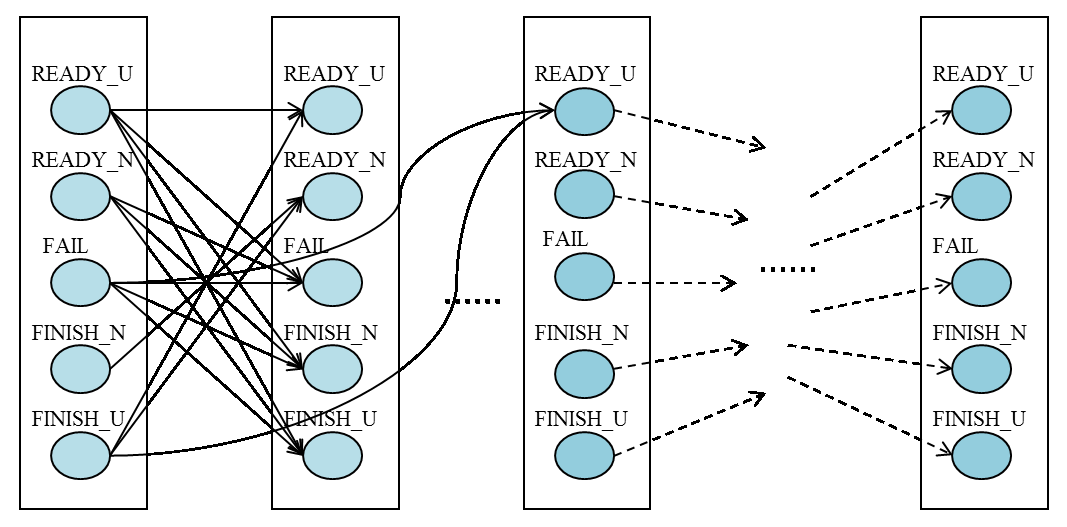
\includegraphics[width = 0.7\textwidth]{ws_state_trans}
    \caption{MDP状态转移图}\label{figure:ws_state_trans}
    \vspace{-1em}
\end{figure}

%\begin{itemize}
%
%\item 时刻~$T$~: 前服务环节执行中/执行后发生不确定事件、或者预知到尚未执行的环节将会发生不确定事件时开始决策,此时为时刻0。如图~\ref{figure:many_utg_tree}~所示的多棵~UTG~连接形成完全触发关系图,叶子结点的状态处于最终时刻~$V$~,“完全触发关系图”的层数是周期个数。这是一个不定周期的时刻序列。
%
%\item 状态~$S$~: 服务前锋线上的所有活动的状态即可表示为服务流程的状态,原因是前锋线上的活动状态已知,则可知所有活动的状态。将服务流程的所有活动的六种状态组成一个状态集合,形成~MDP~状态~$state$~, 即~$state =  < state({a_1}),state({a_2}), \ldots ,state({a_n}) >$~,每个状态附着两个参数(~$T$~和~$C$~);
%
%\item 动作~$A$~:共有终止、不作为、重试、替换、重组五个动作,不同状态下可执行的动作集合有所不同(见表~\ref{table:state_action}~)。
%
%\item 转移概率~$P$~:转移概率由当前的决策动作和服务活动的状态联合决定,即~$p(state_j|state_i,action)$~的值有以下几类情况:
%\begin{itemize}
%    \item ~$1;~if~action = continue/terminate$~
%    \item ~$reliability;~if~action = retry/substitute/re-compose~ \& ~ state_j = FINIS{H^{N/U}}$~
%    \item ~$1 - reliability;~if~action = retry/substitute/re-compose ~\& ~ state_j = FAIL$~
%\end{itemize}
%其中~$reliability$~指的是将要执行的服务端可靠性,若有多个服务,则是多个服务可靠性之积。
%
%\item 报酬函数~$Reward$~:在~\ref{sec:model_section}~节中给出。
%
%\end{itemize}

\paragraph{算法}

基于上述五个方面的基本定义,采用有限阶段向后递归迭代~MDP~算法进行最优决策序列的求解,得到对当前服务的决策动作。

算法:基于~MDP~的服务不确定性优化决策

输入:服务方案~$SPlan$~、与当前发生的不确定性事件相关的活动~$activity$~、
~$SPlan$~中各个活动的当前状态、服务执行的目标状态

输出:最优马氏策略及其成本

步骤~1~~根据出现不确定性的活动~$a$~,按照表~\ref{table:state_action}~构造~UTG~,并将多棵~UTG~连接形成“完全触发关系图”,如图\ref{figure:ws_state_trans}所示,从而形成状态转移表;

步骤~2~~定义当前的不确定状态为时刻0,以此生成向后衍生的UTG,最后一个活动执行结束的时刻为最终时刻V。从而生成0到~$V$~的~$V+1$~个时刻的若干个状态、若干个动作、相应的转移概率报酬;

步骤~3~~令~$t=V$~,且对所有~$V$~时刻的状态~$state_V \in S$~,令~${u_V}( {state_V} ) = Reward_V( {state_V} )$;

步骤~4~~ 如果~$t=0$~,则~$\pi  = (f_0,f_1,\ldots ,f_{V-1})$~为最优的马氏策略,而~${u_0}( state_0)$~为最优的值函数,算法停止。否则,令~$t=t–1$~,进入步骤5;

步骤~5~~ 对所有~$state_t \in S$~,计算

\begin{equation}\label{equation:backward_mdp}
\begin{array}{l}
{u_t}(stat{e_t}) = \mathop {\max }\limits_{action \in Action(stat{e_t})} \{ Rewar{d_t}(stat{e_t},action)\\
{\rm{                        }} + \sum\limits_{stat{e_{t + 1}} \in S} {{p_t}(stat{e_{t + 1}}|stat{e_t},action){u_{t + 1}}(stat{e_{t + 1}})} \} 
\end{array}
\end{equation}

并记集合

\begin{equation}\label{equation:backward_mdp_arg}
\begin{array}{l}
Actio{n_t}(stat{e_t}) = \mathop {\arg \max }\limits_{action \in Action(stat{e_t})} \{ Rewar{d_t}(stat{e_t},action)\\
{\rm{                       }} + \sum\limits_{stat{e_{t + 1}} \in S} {{p_t}(stat{e_{t + 1}}|stat{e_t},action){u_{t + 1}}(stat{e_{t + 1}})} \} 
\end{array}
\end{equation}

任意取~$f_t(state_t) \in Action_t(state_t)$~,于是定义了~$t$~时刻的决策规则~$f_t$~。而0时刻的决策~$f_0$~则是对当前不确定性出现的时刻采取最优的决策动作。

步骤~6~~ 返回步骤3。

\subsection{基于价值的业务层服务不确定性决策}

业务层面的服务不确定性决策的目标可描述为:最大化服务提供者的收益,最小化用户提供的成本,满足用户需求变化和资源得到充分利用。

\subsubsection{服务执行的状态}

针对业务层服务的执行,不仅仅只是一个服务流程在执行,而有多个服务流程一起协作执行,需要评估服务执行的总收益。服务方案仍然如式(\ref{equation:splan})所示。而多个服务同时执行,这服务方案表示为如式(\ref{equation:splanlist})所示。

\begin{equation}\label{equation:splanlist}
SPlan\_LIST = \left(SPlan_1, SPlan_2, ..., SPlan_n\right)
\end{equation}
\begin{tabularx}{\textwidth}{@{}l@{\quad}l@{\pozhehao }X@{}}
    式中
    & ${SPlan_i}$ & 第$i$个服务流程,如式(\ref{equation:splan})所示。
\end{tabularx}\vspace{\wordsep}

业务服务流程中,每一个服务的执行需要依赖其需要的资源,候选资源如式(\ref{equation:c_res})所示。

\begin{equation}\label{equation:c_res}
Resource = \left(id, type, use\_type, price \right)
\end{equation}
\begin{tabularx}{\textwidth}{@{}l@{\quad}l@{\pozhehao }X@{}}
    式中
    & ${id}$ & 资源编号;\\
    & ${type}$ & 资源类型;\\
    & ${use\_ype}$ & 最高并发度,1表示同时只能1个,2表示同时只能2个,以此类推;\\
    & ${price}$ & 资源价格。
\end{tabularx}\vspace{\wordsep}

因此,每一个活动上除了如式(\ref{equation:activity})上所示的软件服务中的参数之外,还有其需要的资源信息,表示为如式(\ref{equation:bs_activity})所示。

\begin{equation}\label{equation:bs_activity}
{a_i} = ({CS_i}, {S_{i0}}, {LST_i}, {LET_i}, {RES\_NEED})
\end{equation}
\begin{tabularx}{\textwidth}{@{}l@{\quad}l@{\pozhehao }X@{}}
    式中
    & ${CS_i}$ & 活动的可替换服务集;\\
    & ${S_{i0}}$ & 当前被选中用于执行该活动$i$的具体服务;\\
    & ${LST_i}$ & 最晚开始时间;\\
    & ${LET_i}$ & 最晚结束时间; \\
    & ${RES\_NEED}$ & 资源需求信息。
\end{tabularx}\vspace{\wordsep}

其资源需求信息则如式(\ref{equation:res_need})所示,表示从开始时间~$BT_i$~到结束时间~$ET_i$~需要资源~${Resource_i}$~。

\begin{equation}\label{equation:res_need}
RES\_NEED = (BT_i, ET_i, Resource_i)
\end{equation}
\begin{tabularx}{\textwidth}{@{}l@{\quad}l@{\pozhehao }X@{}}
    式中
    & ${BT_i}$ & 开始时间;\\
    & ${ET_i}$ & 结束时间;\\
    & ${Resource_i}$ & 资源信息,如式(\ref{equation:c_res})所示。
\end{tabularx}\vspace{\wordsep}

\subsubsection{决策动作}

在业务层面,服务的不确定性事件除了软件层面的不确定性事件之外,还有以下四种不确定性事件:
\begin{itemize}
    \item 资源不可用,指服务执行所依赖的资源在某个时间段不能提供,服务无法正常执行;
    \item 需求增加,指某个流程的用户增加需求,需要额外的资源才能满足;
    \item 需求减少,指某个流程的用户需求比预定的减少,造成资源的浪费;
    \item 需求取消,指某个流程用户取消预定的需求,服务流程不需要继续执行。
\end{itemize}

针对这几种不确定性,总结出5种对应的动作。

\begin{itemize}
    \item 资源替代,指采用候选的资源对当前出现不确定性的资源进行替换,原服务可以得以继续执行;
    \item 资源迁移,指将正常执行的流程上的资源迁移到出现不确定性的服务流程上,出现不确定性的流程得以正常执行,但是引入新的代价则是此原来可以正常执行的服务不能继续执行;
    \item 终止需求,指终止用户的需求,不进行响应;
    \item 不作为,指对出现的不确定性事件视而不见的鸵鸟做法;
    \item 引入~$m+k$~个新需求,指资源出现浪费的时候,引入新的需求来避免资源浪费。
\end{itemize}

举一个例子,淘宝店主的货物,可以通过不同的快递公司发到顾客手里。但是期间可能出现某个快递公司临时不能提供快递服务(资源不可用),或者某个用户临时增加订单(需求增加)/减少订单(需求减少)/取消订单(需求取消),则淘宝店主需要根据不同的不确定性事件采取不同的决策动作,以保证自身业务的正常运行。例如新签约其他的快递公司(资源替代),对某些不紧急的货物延迟发货而把它的快递资源迁移给一些紧急的货物运输上(资源迁移),不满足用户新增的订单需求(终止需求),对快递公司出现的不确定性采取不作为手段使得快递公司自己去解决(不作为)。

\subsubsection{决策收益(价值)}

在业务层服务执行出现不确定性,每一个动作可能带来~4~个效应:

\begin{itemize}
    \item 引入新成本~$\Delta C_{new}$,指资源替换将引入新的资源时所带来的成本消耗;
    \item 资源迁移成本~$\Delta C_{trans}$,指资源从一个流程上迁移到另一个流程所需要的成本消耗;
    \item 已经使用的资源成本~$\Delta C_{used}$,指在不确定性活动上预分配的成本,服务执行已经消耗后无法追回的成本;
    \item 失败赔偿~$\Delta C_{p}$,指在不确定性活动上预分配的成本,服务执行已经消耗后无法追回的成本。
\end{itemize}

因此,在衡量决策收益时,则是这几个成本消耗之和的负值。如式(\ref{equation:bs_reward})所示。

\begin{equation}\label{equation:bs_reward}
reward_{bs} = - (\Delta C_{new} + \Delta C_{trans} + \Delta C_{used} + \Delta C_{p})
\end{equation}

软件层服务不确定性和业务层服务不确定性同时存在则是普遍意义上服务的不确定性,因此,由于资源的替换或者转移不影响原服务的执行可靠性,因此在业务层服务不确定性的决策时不考虑服务成功执行的概率,而将此部分放在软件层服务不确定性的决策中。

与软件层服务不确定性类似的,对不同的不确定性事件需要采取不同的决策动作,不同的动作则带来不同的收益。因此,业务层服务不确定性事件、决策动作和收益之间的关系如表~\ref{table:state_action_business}~所示。

% Table generated by Excel2LaTeX from sheet 'Sheet9'
\begin{table}[htbp]
    \caption{业务层面服务不确定性决策}
    \vspace{-0.5em}\label{table:state_action_business}\centering\zihao{5}
    \begin{threeparttable}
        \begin{tabular}{lllllll}
            %    \begin{tabularx}{\textwidth}{llXlllll}
            \toprule
            % Header
            & \multicolumn{1}{c}{不确定性事件} 
            & \multicolumn{1}{c}{{决策动作}} 
            & \multicolumn{1}{c}{$\Delta C_{new}$} 
            & \multicolumn{1}{c}{$\Delta C_{trans}$} 
            & \multicolumn{1}{c}{$\Delta C_{used}$} 
            & \multicolumn{1}{c}{$\Delta C_{p}$} \\
            \hline

            & \multicolumn{1}{c}{资源不可用} 
            & \multicolumn{1}{c}{资源替代} 
            & \multicolumn{1}{c}{$price_{ijk}$\tnote{1}} 
            & \multicolumn{1}{c}{0} 
            & \multicolumn{1}{c}{$price_{ij0}$\tnote{2}} 
            & \multicolumn{1}{c}{0} \\
            
            & \multicolumn{1}{c}{} 
            & \multicolumn{1}{c}{资源迁移} 
            & \multicolumn{1}{c}{0} 
            & \multicolumn{1}{c}{$\sum\limits_{k = 0}^m {price\_tran{s_{ijk}}}$ \tnote{3}}
            & \multicolumn{1}{c}{$price_{ij0}$}
            & \multicolumn{1}{c}{$price\_p_i$ \tnote{4}} \\
            
            & \multicolumn{1}{c}{} 
            & \multicolumn{1}{c}{终止需求} 
            & \multicolumn{1}{c}{0} 
            & \multicolumn{1}{c}{0} 
            & \multicolumn{1}{c}{$\sum\limits_{j \in SPla{n_i}} {pric{e_j}}$\tnote{5}} 
            & \multicolumn{1}{c}{$price\_p_i$} \\
            
            & \multicolumn{1}{c}{需求增加} 
            & \multicolumn{1}{c}{资源替代} 
            & \multicolumn{1}{c}{$price_{ijk}$} 
            & \multicolumn{1}{c}{0} 
            & \multicolumn{1}{c}{$price_{ij0}$} 
            & \multicolumn{1}{c}{0} \\
            
            & \multicolumn{1}{c}{} 
            & \multicolumn{1}{c}{资源迁移} 
            & \multicolumn{1}{c}{0} 
            & \multicolumn{1}{c}{$\sum\limits_{k = 0}^m {price\_tran{s_{ijk}}}$}
            & \multicolumn{1}{c}{$price_{ij0}$}
            & \multicolumn{1}{c}{$price\_p_i$} \\
            
            & \multicolumn{1}{c}{} 
            & \multicolumn{1}{c}{不作为} 
            & \multicolumn{1}{c}{0} 
            & \multicolumn{1}{c}{0} 
            & \multicolumn{1}{c}{0} 
            & \multicolumn{1}{c}{$price\_p_i$} \\
            
            & \multicolumn{1}{c}{需求减少} 
            & \multicolumn{1}{c}{不作为} 
            & \multicolumn{1}{c}{0} 
            & \multicolumn{1}{c}{0} 
            & \multicolumn{1}{c}{$price_{ij0}$} 
            & \multicolumn{1}{c}{0} \\
            
            & \multicolumn{1}{c}{} 
            & \multicolumn{1}{c}{引入$m+k$个新需求} 
            & \multicolumn{1}{c}{0} 
            & \multicolumn{1}{c}{0} 
            & \multicolumn{1}{c}{0} 
            & \multicolumn{1}{c}{$-\sum\limits_{j = SPla{n_m}}^{SPla{n_k}} {price\_{p_j}}$} \\
            
            & \multicolumn{1}{c}{需求取消} 
            & \multicolumn{1}{c}{终止需求} 
            & \multicolumn{1}{c}{0} 
            & \multicolumn{1}{c}{0} 
            & \multicolumn{1}{c}{$\sum\limits_{j \in SPla{n_i}} {pric{e_j}}$} 
            & \multicolumn{1}{c}{0} \\
            
            & \multicolumn{1}{c}{} 
            & \multicolumn{1}{c}{引入$m+k$个新需求} 
            & \multicolumn{1}{c}{0} 
            & \multicolumn{1}{c}{0} 
            & \multicolumn{1}{c}{0} 
            & \multicolumn{1}{c}{$-\sum\limits_{j = SPla{n_m}}^{SPla{n_k}} {price\_{p_j}}$\tnote{6}} \\
            
            \bottomrule
            
        \end{tabular}%
        \begin{tablenotes}
            \item[1] $price_{ijk}$~表示价格,其下标分别表示第~$i$~个流程,第~$j$~个活动,$k$~是替换后的新资源编号;
            \item[2] $price_{ij0}$~表示价格,其下标分别表示第~$i$~个流程,第~$j$~个活动,$0$~是替换前的旧资源编号;
            \item[3] $\sum\limits_{k = 0}^m {price\_tran{s_{ijk}}}$~表示~$0-m$~个资源从服务流程~$i$~迁移到服务流程~$j$~上的迁移成本;
            \item[4] $price\_p_i$~表示第~$i$~个服务流程执行失败时的赔偿价格;
            \item[5] $\sum\limits_{j \in SPla{n_i}} {pric{e_j}}$~表示第~$i$~个服务流程执行失败时,其所有活动上绑定的资源成本;
            \item[6] $-\sum\limits_{j = SPla{n_m}}^{SPla{n_k}} {price\_{p_j}}$~表示~$m$~到~$k$~个新服务流程成功执行获得的新收益,与成本是反方向,故为负值。
        \end{tablenotes}
    \end{threeparttable}
\end{table}%

\subsubsection{业务层不确定性决策算法}

在以上介绍的业务层服务不确定性的5个决策动作中,资源迁移算法需要抽取成为为一个子算法,来计算如何迁移资源获得的收益最大(赔偿最小)。子算法嵌入到业务层不确定性决策算法的主算法中,完成整体算法。

\setcounter{paragraph}{0}
\paragraph{资源迁移算法(最小代价区间覆盖)}

在服务流程出现不确定性的活动上,实际上是在一个时间区间~$[b,e]$~上的资源能提供给服务执行所用,而需要从别的服务流程的活动上的资源迁移到这个活动上。同样,别的服务流程活动上的资源也是在一个时间区间内有效。动作则是将多个活动上的资源进行迁移,使得资源在时间~$[b,e]$~上有效,从而完成资源迁移的目的。

如何进行资源迁移,使得代价最小,这即转化成了最小代价区间覆盖问题:有~$n$~个区间,求覆盖~$[b,e]$~的最小代价,每个区间的代价为~$price\_trans_i ~(0 \le i \le n)$~。

很显然,这是一个动态规划问题,~$f[i]$~表示取~$[b,i]$~这个区间的代价,显然~$f[b-1]=0$,所求的解为~$f[e]$~。则转移方程如式(\ref{equation:dp_trans})所示。

\begin{equation}\label{equation:dp_trans}
f[a[i].{t_2}] = \mathop {\min }\limits_{({t_1} - 1 \le j \le {t_2} - 1)} (f[j]) + a[i].price\_trans
\end{equation}

从而得到资源迁移算法,如算法\ref{alg1}所示。
%
%输入:区间个数~$n$~,$n$~个区间~$data$~, 即~$[t_{1}, t_{2}]$~,$n$~个转移代价~$price\_trans$~
%
%输出:选择方案,最小代价~$minCost$~

\begin{algorithm}
    \caption{最小代价区间覆盖}
    \label{alg1}
    \begin{algorithmic}
        \STATE 输入:区间个数~$n$~, $n$~个区间~$data[n]$~
        \STATE 输出:最小代价~$minCost$~
        \STATE sort $data$ by $t_2$;
        \IF{$b < data[0].t_1 ~\OR~ e > data[n-1].t_2$}
            \STATE return $-1$;
        \ENDIF
        \FOR{$i=1$ to $n$}
            \IF{$data[i].t2 \ge b ~\AND~ data[i].t1 \le b$}
            \STATE $first \Leftarrow i$
            \STATE break;
            \ENDIF
        \ENDFOR
        
        \FOR{$i=1$ to $data[first].t_1-1$}
            \STATE $f[i] \Leftarrow 0$
        \ENDFOR
        
        \FOR{$i=first$ to $n$}
            \IF{$data[i].t_2 < b$}
                \STATE continue;
            \ENDIF
            \FOR{$j=data[i].t_1-1$ to $data[i].t_2-1$}
                \STATE $f[i] \Leftarrow 0$
                \STATE $t_{1min} = \min(t_{1min}, f[j])$
            \ENDFOR
            \STATE $f[data[i].t_2] = \min (f[data[i].t_2], t_{1min} + data[i].price)$
        \ENDFOR
        \STATE return $f[e]$

    \end{algorithmic}
\end{algorithm}

%步骤~1~~ 将区间按照右端点从小到大排序;
%
%步骤~2~~ 若 ~$b < data[1].t_1$ 或 ~$e > data[n].t_2$,无法覆盖,退出;
%
%步骤~3~~ 寻找第一个比~$b$~大的区间~$first$~,将~$f[0] - f[first]$~初始化为0;
%
%步骤~4~~ 对于从~$first$~取到~$n$~的区间~$i$~,按照式(\ref{equation:dp_trans})计算;
%
%步骤~5~~ 构造资源选择代价为~$f[e]$~的选择方案,输出~$f[e]$~和选择方案。


\paragraph{不确定性决策算法(贪心策略)}

业务层服务不确定性算法采用贪心策略,一旦发生不确定性事件,立刻根据不同的不确定性事件采取不同的决策动作,计算需要的代价,选择最小的代价动作作为不确定性的决策动作。

输入:不确定性事件~$event$,当前~$m$~个服务流程状态

输出:最优的不确定性决策动作

步骤~1~~ 根据不确定性事件类型,查表\ref{table:state_action_business}选择相应的不确定性动作;

步骤~2~~ 如果相应的不确定性动作有“资源迁移”,则对每一个流程~$j (j \neq i)$~,采用算法\ref{alg1}计算资源迁移代价,选择最小的迁移代价作为“资源迁移”动作的代价;

步骤~3~~ 根据表\ref{table:state_action_business}计算不同动作的代价;

步骤~4~~ 输出最小代价的动作。


\subsection{支持不确性决策的仿真系统}

业务层面服务不确定性决策和软件层面服务不确定性决策有几点不同:

\begin{itemize}
    \item 不确定性事件的类型不同,由此带来的决策动作也不同。业务层面面向的是服务资源和用户需求的不确定性事件,而软件层面面向软件服务本身的不确定性事件;
    \item 软件层面面向一个服务流程,而业务层面面向多个服务流程。软件层面面向一个服务流程进行最优化决策,而业务层面则是多方协作整体最优化决策;
    \item 软件层面的不确定性会往后传播,影响到后面活动的正常执行,而业务层面的不确定性很难衡量往后传播的特性,例如:用户需求发生变化是完全不可预知的,也无法衡量其向后的影响。
\end{itemize}

因此,针对软件层和业务层的服务不确定性,开发出一个不确定性仿真系统,支持软件层面和业务层面的服务不确定性仿真。此系统将采用随机的不确定性事件产生器,仿真执行将预定义的组合服务流程。

\subsubsection{系统架构}

系统进行仿真的时候,选服务集(包括服务的QoS)随机生成,不确定性事件由正在执行的服务的可靠性提供概率作为生成种子。例如,目前正在执行的活动上绑定的服务的可靠性为~$r$~,则系统以$(1-r)$的概率产生不确定性事件。

仿真系统结构如图~\ref{figure:sim_structure}~所示,整个仿真系统有一个流程执行控制器控制执行过程,不确定性事件产生器根据流程控制器当前的执行状态信息(例如可靠性)产生不确定性事件,更新到界面上显示,同时立刻采用修复算法修复,得到新的流程信息,更新到界面上,界面的信息反馈到流程执行控制器,流程执行控制器继续执行。如此往复。

系统的输入:~Web Service~执行方案、资源方案。

系统的输出:仿真输出服务执行的整个过程。

\begin{figure}[htbp]
    \centering
    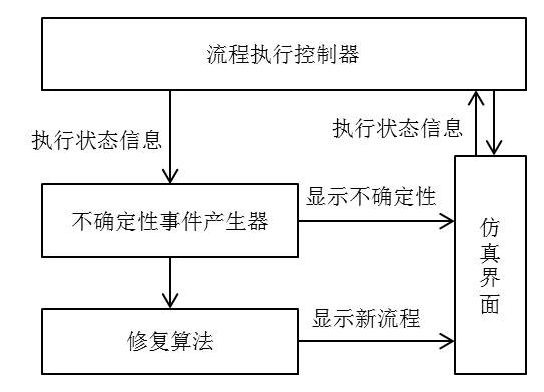
\includegraphics[width = 0.5\textwidth]{sim_structure}
    \caption{支持不确定性决策的仿真系统结构}\label{figure:sim_structure}
    \vspace{-1em}
\end{figure}

\subsubsection{详细设计}

仿真系统需要完成两个功能:运行仿真程序、监听数据变化刷新仿真界面。很显然一个线程无法同时完成两个不同的功能。因此,设计两个线程,主线程用于界面控制,子线程用于仿真程序。子线程和主线程之间进行数据共享,确保主线程显示的数据为子线程仿真程序的数据,同时主线程的界面操作也返回到子线程的仿真程序中。其详细设计如图\ref{figure:sim_detail}所示。

\begin{figure}[htbp]
    \centering
    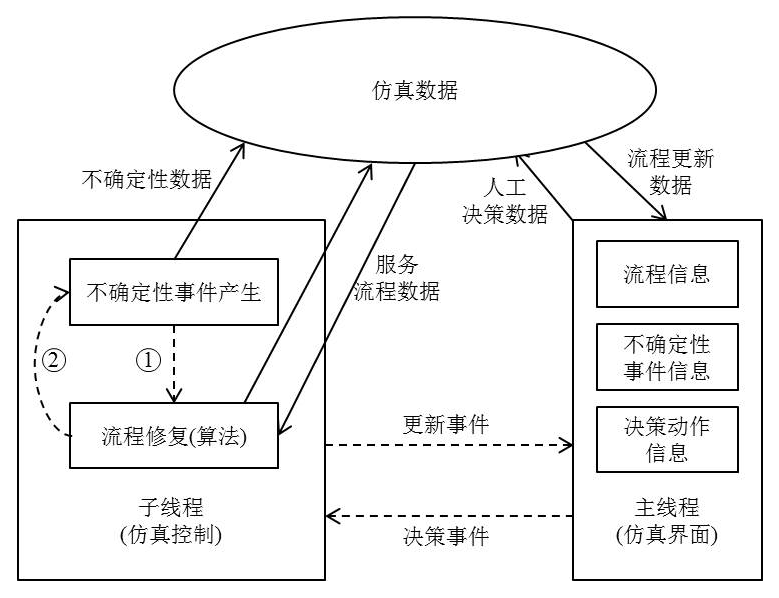
\includegraphics[width = 0.65\textwidth]{sim_detail}
    \caption{支持不确定性决策的仿真系统详细设计}\label{figure:sim_detail}
    \vspace{-1em}
\end{figure}

仿真系统提供~2~个仿真功能:

(1)~自动仿真,指的是不在人为的干预下,仿真执行服务流程的过程,一旦发生不确定性事件,由算法自动采取最优决策,修复服务流程后继续执行,如此往复,直至服务流程执行结束;

(2)~人工仿真,指的是在自动仿真服务流程执行过程,一旦不确定性事件产生,算法给出多个应对不确定性事件的决策动作,由人工选择决策动作(不一定选择最优决策),仿真系统根据选择的动作修复服务流程,之后继续执行,如此往复,直至服务流程执行结束。

自动仿真的主程序的运行步骤为:

(1)~主线程开始运行,初始化仿真界面;

(2)~新建子线程;

(3)~子线程读入配置文件、服务信息,并初始化;

(4)~子线程开始仿不确定性仿真,进入循环体;

(5)~子线程判断仿真是否结束,结束则跳至第~(9)~步,否则下一步;

(6)~子线程不确定性事件产生器产生不确定性事件;

(7)~子线程算法自动产生最优的决策动作,根据决策动作修复服务流程;

(8)~返回第~(5)~步。

(9)~子线程退出,主线程在人工关闭仿真界面后退出。

人工仿真的主程序的运行步骤为:

(1)~主线程开始运行,初始化仿真界面;

(2)~新建子线程;

(3)~子线程读入配置文件、服务信息,并初始化;

(4)~子线程开始仿不确定性仿真,进入循环体;

(5)~子线程判断仿真是否结束,结束则跳至第~(10)~步,否则下一步;

(6)~子线程不确定性事件产生器产生不确定性事件,阻塞子线程,等待主线程反馈;

(7)~主线程等待人工操作界面选择决策动作,将选择结果返回给子线程,若无人工选择,一直等待;

(8)~子线程根据主线程返回的决策动作修复服务流程;

(9)~返回第~(5)~步。

(10)~子线程退出,主线程在人工关闭仿真界面后退出。

由于主线程和子线程之间有大量的数据需要同步,因此在程序适当的地方需要加锁。

\subsubsection{系统开发}

系统开发采用的开发环境:~C++~语言,Qt~框架,编译器为~gcc 4.4,版本控制采用~Git~,代码托管至~github.com~;

运行环境:系统平台~Microsoft Windows 7 64bit, 处理器为~Intel® ~Core i3 CPU 3.0GHz~,系统内存为~4G~。

由于~C++~和~Qt~框架的跨平台特性,系统也具备跨平台特性,只需在不同的平台重新编译即可运行在不同的平台,例如~Lnux~、Mac OS~。

系统开发分为软件层面和业务层面,首先对软件层面的不确定性进行自动仿真。

如图\ref{figure:ws_sim}所示,左上角为服务执行流程,每一个圆圈代表一个活动,活动以三种颜色标识其执行状态,绿色表示就绪态,红色表示出现不确定性事件,蓝色表示执行完成。仿真的过程可以看到不断的红色的活动出现,但是其可以看到算法自动采取决策动作,之后修复服务流程,以此往复,直至图中所有的点变成蓝色而结束。

如图\ref{figure:ws_sim}的服务流程的每个活动上绑定有执行的服务,其服务信息如图的右上角部分所示,产生的的不确定性如左下角所示,同时将发生的不确定性和采取的动作也记录到左下角显示。右下角提供算法算出的决策动作,以及其带来的直接收益、潜在收益、成本消耗、时间延迟、成功执行的概率等信息。其中,直接收益指的是通过贪心算法算出,而潜在收益则是根据~MPD~算法给出,可以看到不同的算法给出的代价不一样,自动仿真则自动选择最优潜在收益的动作进行仿真。

\begin{figure}[htbp]
    \centering
    \includegraphics[width = 1.0\textwidth]{ws_sim}
    \caption{支持服务不确定性决策仿真系统(软件层面)}\label{figure:ws_sim}
    \vspace{-1em}
\end{figure}

软件服务流程也支持人工仿真,人工仿真则是仿真系统自动算出多个决策动作所带来的收益,包括直接收益、潜在收益、成本消耗、时间延迟、成功执行的概率等信息,由人工选择理想的决策动作,而不一定是最优的决策动作进行仿真。例如,当出现如图\ref{figure:ws_sim_manual_event}所示的不确定性事件后,系统得到四个决策动作以及其带来的收益如图\ref{figure:ws_sim_manual_action}所示,当人工选择一个决策动作之后,会弹出窗口再次确认决策动作的信息,以及其可能造成后续活动失败等的潜在风险说明。当人工选择“OK”时,服务流程按照人工选择的决策动作进行修复,继续仿真,如此往复,直至结束。

\begin{figure}[htbp]
    \centering
    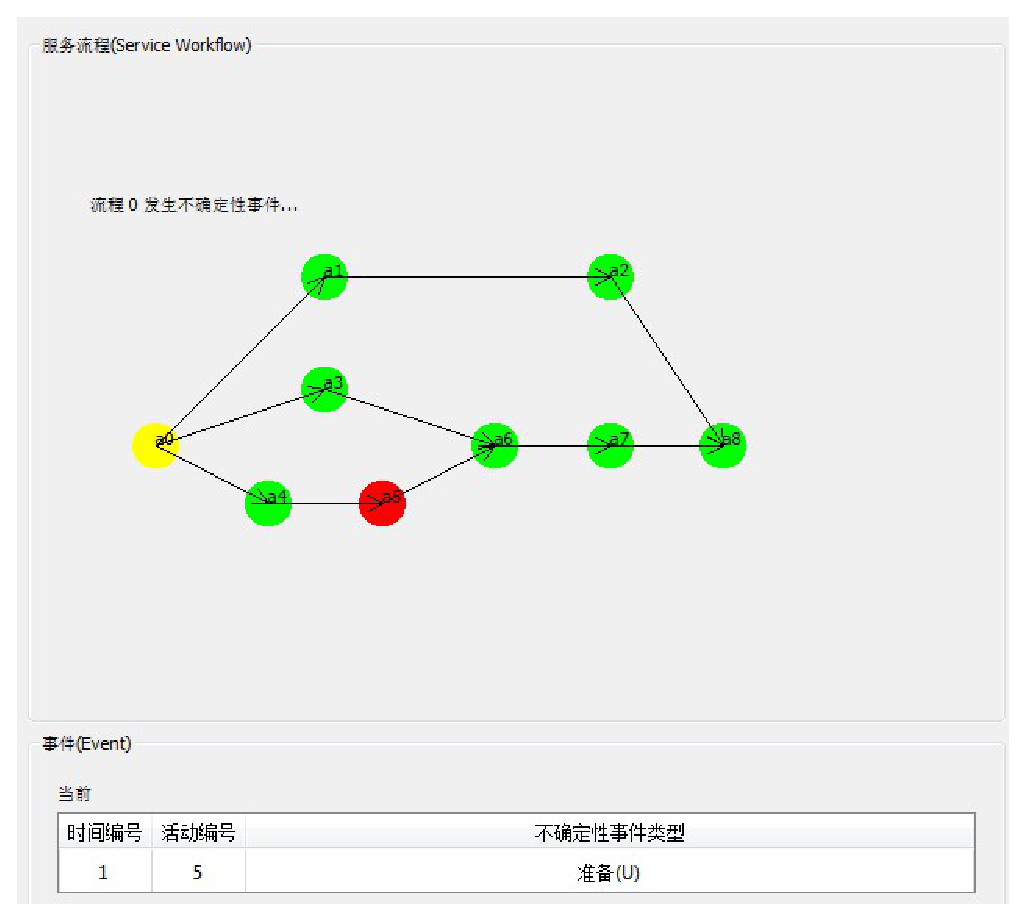
\includegraphics[width = 0.7\textwidth]{ws_sim_manual_event}
    \caption{支持服务不确定性决策仿真系统(软件层面不确定性事件)}\label{figure:ws_sim_manual_event}
    \vspace{-1em}
\end{figure}


\begin{figure}[htbp]
    \centering
    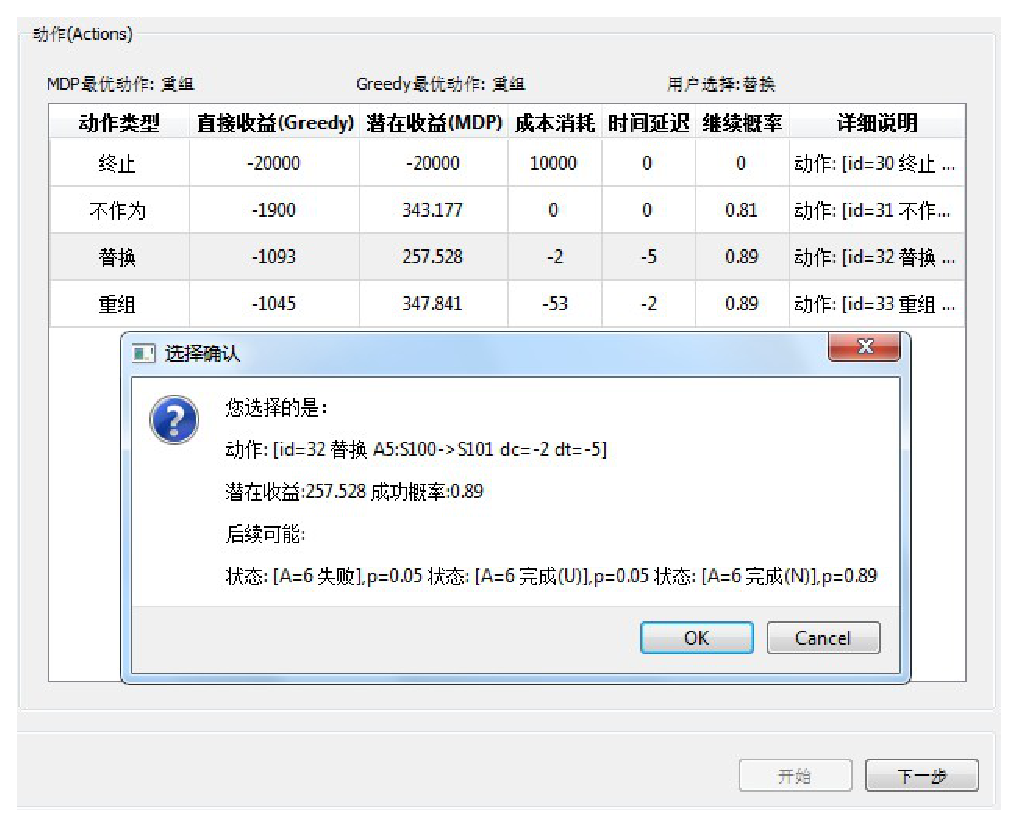
\includegraphics[width = 0.7\textwidth]{ws_sim_manual_action}
    \caption{支持服务不确定性决策仿真系统(软件层面人工决策)}\label{figure:ws_sim_manual_action}
    \vspace{-1em}
\end{figure}

对于业务服务的不确定性仿真,则是针对多个服务流程同时执行,如图\ref{figure:bs_sim}所示,上半部分为服务执行流程,有~8~个同时执行。同样,每一个圆圈代表一个活动,活动以三种颜色标识其执行状态,绿色表示就绪态,红色表示出现不确定性事件,蓝色表示执行完成。仿真的过程可以看到不断的红色的活动出现,但是其可以看到算法自动采取决策动作,之后修复服务流程,以此往复,直至图中所有的点变成蓝色而结束。中间部分为服务绑定的资源信息,包括编号、价格。左下部分是产生的不确定性事件以及发生不确定性后采取的决策动作历史记录。

\begin{figure}[htbp]
    \centering
    \includegraphics[width = 1.0\textwidth]{bs_sim}
    \caption{支持服务不确定性决策仿真系统(业务层面)}\label{figure:bs_sim}
    \vspace{-1em}
\end{figure}

同样,软件服务流程也支持人工仿真,人工仿真则是仿真系统自动算出多个决策动作所带来的收益,由人工选择理想的决策动作,而不一定是最优的决策动作进行仿真。例如,当出现如图\ref{figure:bs_flow}所示的不确定性事件,流程~8~的第~7~号活动发生不确定性事件,系统得到两个决策动作以及其带来的收益如图\ref{figure:bs_action}所示,当人工选择一个决策动作之后,会弹出窗口再次确认决策动作的信息,当人工选择“OK”时,服务流程按照人工选择的决策动作进行修复,继续仿真,如此往复,直至结束。

\begin{figure}[htbp]
    \centering
    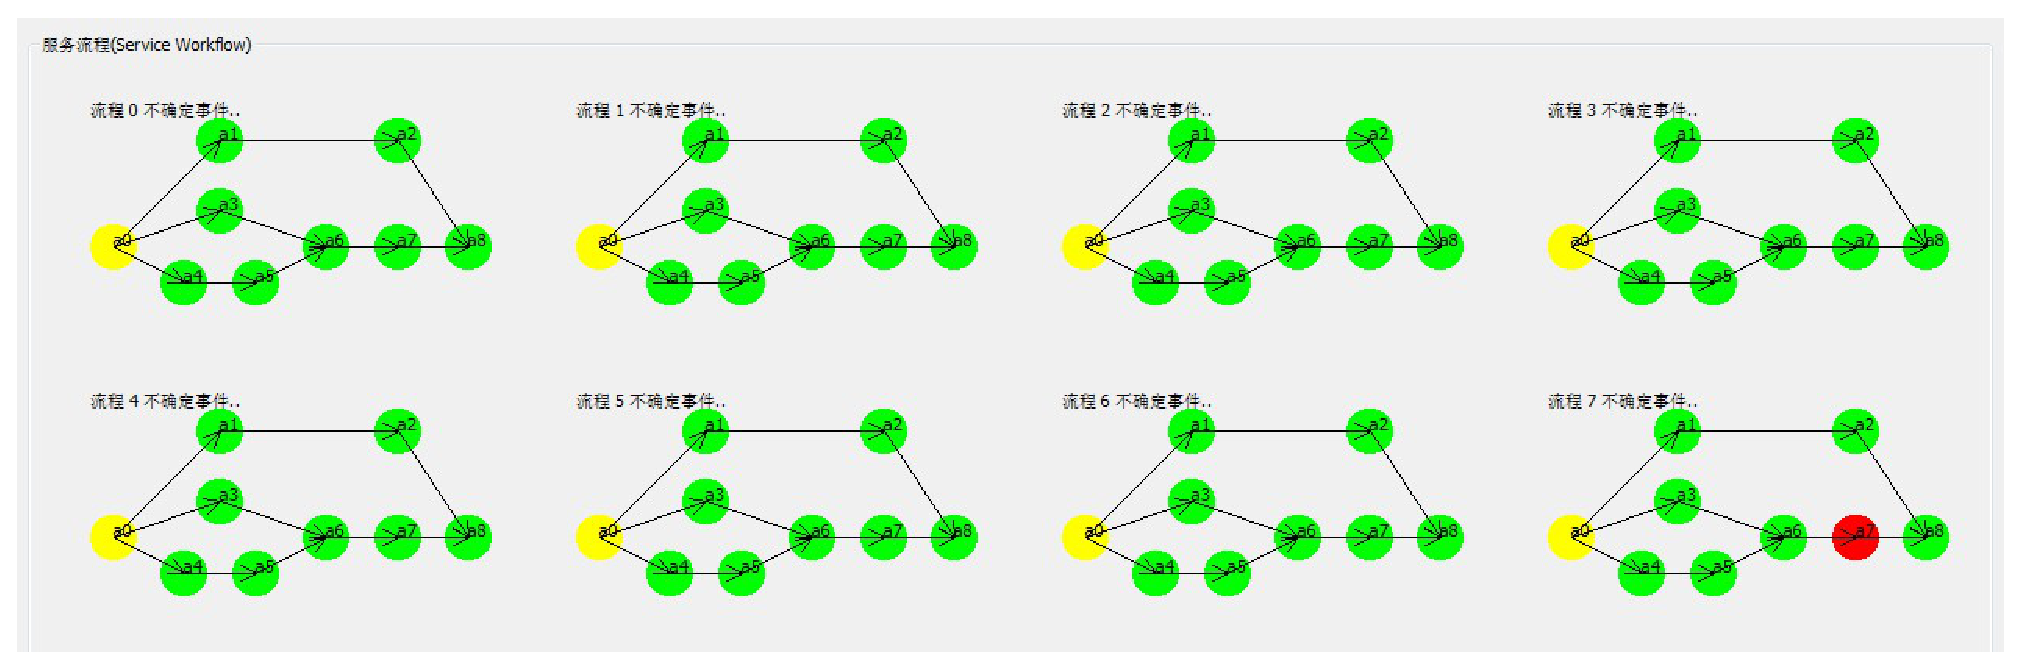
\includegraphics[width = 1.0\textwidth]{bs_flow}
    \caption{支持服务不确定性决策仿真系统(业务层面不确定性事件)}\label{figure:bs_flow}
    \vspace{-1em}
\end{figure}


\begin{figure}[htbp]
    \centering
    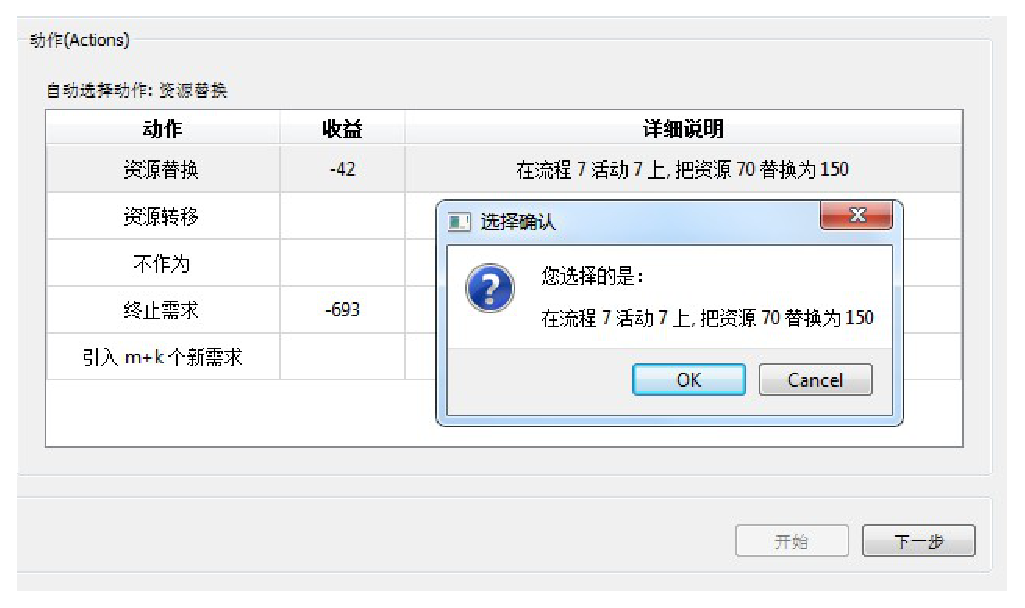
\includegraphics[width = 0.7\textwidth]{bs_action}
    \caption{支持服务不确定性决策仿真系统(业务层面人工决策)}\label{figure:bs_action}
    \vspace{-1em}
\end{figure}

%拟采用的开发环境:Java语言,JDK 1.7; 运行环境:JRE 1.7 64bit,系统平台Microsoft Windows 7 64bit, 处理器为Intel® Core i3 CPU 3.0GHz,系统内存为4G,JVM分配512M内存。



%
%\subsubsection{不确性决策在海运物流中的应用验证}
%
%在基于价值的服务不确定性建模,并在软件服务中得以仿真实验后,以此思路将不确定性决策应用于海运物流业务服务中。因此,需要针对海运物流业务收取相应的信息,对海运物流服务方案、海运物流服务不确定性事件、海运物流服务的执行的状态、海运物流服务决策动作、海运物流服务中事件和决策及状态之间的关系、海运物流服务决策收益进行建模,最后开发出海运物流业务的不确定性决策系统。
%
%\setcounter{paragraph}{0}
%\paragraph{海运物流服务方案}
%
%%此处需要增加业务描述的QoS,需求等等
%%
%%业务层面的服务不同于如式(~\ref{equation:cs}~)所示的表示方式,其除了软件层面的QoS之外,还具备
%
%业务层面的不确定性采用海运物流业务作为示例,其多方之间的工作流程如图~\ref{figure:bp_example}~所示。它实际上就是一个有向图,将其简化转换之后如图~\ref{figure:bp_ws_process}~所示。
%
%\begin{figure}[htbp]
%    \centering
%    \includegraphics[width = 0.95\textwidth]{bp_example}
%    \caption{海运物流工作流}\label{figure:bp_example}
%    \vspace{-1em}
%\end{figure}
%
%\begin{figure}[htbp]
%    \centering
%    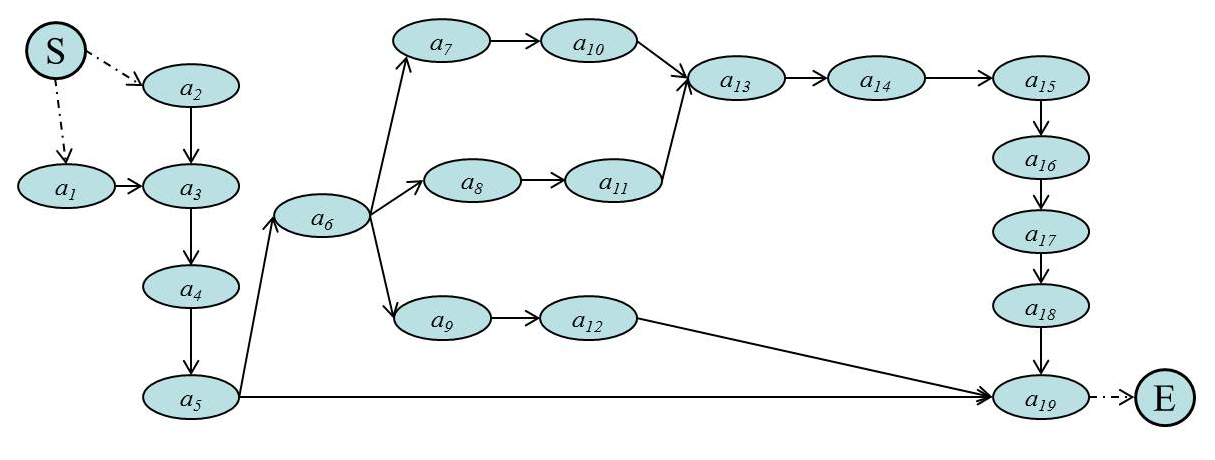
\includegraphics[width = 0.7\textwidth]{bp_ws_process}
%    \caption{海运物流业务DAG图}\label{figure:bp_ws_process}
%    \vspace{-1em}
%\end{figure}
%
%\paragraph{海运物流服务不确定性事件}
%
%业务层面执行比软件层面有更多复杂的不确定性事件,其表示方式如式(\ref{equation:event})所示。其不确定性事件的类型除了软件服务的不确定性事件之外,还增加两类事件:
%
%\begin{itemize}
%    
%    \item 由用户产生的事件,主要指用户需求发生变化,分为以下几类:
%    
%    $E_{31}$:~用户所需~QoS~发生变化,包括执行时间,成本(价格),可靠性等等。
%    
%    $E_{32}$:~用户所需服务发生变化,主要指某个活动用户需要指定某个服务来执行,或者指定不能由某个服务来执行。
%    
%    $E_{33}$:~用户要求终止服务执行。
%    
%    \item 由服务执行方产生的事件,主要指服务执行所需的可用资源发生变化,比如海运物流中集装箱的个数由于损坏而变少,则海运无法继续按照原计划执行运输,再如航空领域由于天气原因导致的航班取消,导致于当天能够起飞的飞机数量变少(甚至于减少为0)。这两类统称为服务的可用资源发生变化,分为以下若干小类:
%    
%    $E_{41}$:~服务所依赖的资源减为0或者完全失效,导致于依赖于此类资源的服务完全不能执行。比如海运物流中,所承载运输的船坏了,所运输的所有物品都不能运输了。
%    
%    $E_{42}$:~服务所依赖的资源减少一部分,导致于服务依赖的资源不足,服务执行受到影响,但不是完全不能执行。比如海运物流中,舱位个数预留不足,导致于货物不能全部装上,此时只能寻找其他船只的舱位同时运输。
%    
%    
%\end{itemize}
%
%其不确定性事件在不同的活动中是不一样的,因此枚举所有活动中所有可能的不确定性事件如表~\ref{table:ocean_shipping_uc}~所示。
%
%% Table generated by Excel2LaTeX from sheet 'Sheet8'
%%\begin{table}[htbp]
%%    \caption{海运物流中的不确定性}
%%    \vspace{-0.5em}\label{table:ocean_shipping_uc}\centering\zihao{5}
%%    \begin{tabular}{cccc}
%%         \toprule
%%         活动编号  & 活动描述  & 需求的不确定性 & 可用资源的不确定性 \\
%%         \midrule
%%         ~$a_1$~ & 发布航线信息 & -     & ~$E_{41}$~ ~$E_{42}$~ \\
%%         ~$a_2$~ & 询问航线信息 & -     & ~$E_{41}$~ ~$E_{42}$~ \\
%%         ~$a_3$~ & 查询、返回航线信息 & ~$E_{31}$~ ~$E_{32}$~ & ~$E_{41}$~ ~$E_{42}$~ \\
%%         ~$a_4$~ & 预订舱位  & ~$E_{31}$~ ~$E_{32}$~ & - \\
%%         ~$a_5$~ & 接受舱位预订 & -     & ~$E_{41}$~ ~$E_{42}$~ \\
%%         ~$a_6$~ & 接受提单  & ~$E_{31}$~ ~$E_{32}$~ & ~$E_{41}$~ ~$E_{42}$~ \\
%%         ~$a_7$~ & 预订集装箱 & ~$E_{31}$~ ~$E_{32}$~ & - \\
%%         ~$a_8$~ & 预订卡车  & ~$E_{31}$~ ~$E_{32}$~ & - \\
%%         ~$a_9$~ & 报关申请  & ~$E_{31}$~   & - \\
%%         ~$a_{10}$~ & 确认集装箱预订 & -     & ~$E_{41}$~ ~$E_{42}$~ \\
%%         ~$a_{11}$~ & 确认卡车预订 & -     & ~$E_{41}$~ ~$E_{42}$~ \\
%%         ~$a_{12}$~ & 报关检查  & -     & ~$E_{41}$~ \\
%%         ~$a_{13}$~ & 运输空箱  & ~$E_{31}$~ ~$E_{32}$~ & ~$E_{41}$~ ~$E_{42}$~ \\
%%         ~$a_{14}$~ & 装载货物进集装箱 & -     & ~$E_{41}$~ ~$E_{42}$~ \\
%%         ~$a_{15}$~ & 铅封集装箱 & ~$E_{32}$~   & ~$E_{41}$~ \\
%%         ~$a_{16}$~ & 运输重箱  & -     & ~$E_{41}$~ ~$E_{42}$~ \\
%%         ~$a_{17}$~ & 堆存货物  & ~$E_{31}$~ ~$E_{32}$~ & ~$E_{41}$~ ~$E_{42}$~ \\
%%         ~$a_{18}$~ & 货物装船  & ~$E_{31}$~ ~$E_{32}$~ & ~$E_{41}$~ ~$E_{42}$~ \\
%%         ~$a_{19}$~ & 运输货物至目的地 & -     & ~$E_{41}$~ \\
%%         \bottomrule
%%    \end{tabular}%
%%\end{table}%
%
%\begin{table}[htbp]
%    \caption{海运物流中的不确定性}
%    \vspace{-0.5em}\label{table:ocean_shipping_uc}\centering\zihao{5}
%    \begin{tabularx}{\textwidth}{cX}
%        \toprule
%        活动编号  & \multicolumn{1}{c}{可能的不确定性} \\
%        \midrule
%        ~$a_1$~ & ~$E_{41}$:(天气原因)轮船不能航行;~$E_{42}$:(轮船损坏)轮船数量减少; \\
%        ~$a_2$~ & ~$E_{41}$:(天气原因)轮船不能航行;~$E_{42}$:(轮船损坏)轮船数量减少; \\
%        ~$a_3$~ & ~$E_{31}$:需求的价格/运输时间/可靠性发生变化;~$E_{32}$:用户指定需要某(种)条船;~$E_{41}$:轮船不能航行;~$E_{42}$:轮船数量减少; \\
%        ~$a_4$~ & ~$E_{31}$:需求的价格发生变化;~$E_{32}$:用户指定需要某个(种)舱位; \\
%        ~$a_5$~ & ~$E_{41}$:(海关原因)舱位完全不能满足;~$E_{42}$:(轮船损坏)能提供的舱位数量不足; \\
%        ~$a_6$~ & ~$E_{31}$:需求的价格发生变化;~$E_{32}$:用户指定需要某个/种舱位;~$E_{41}$:舱位完全不能满足;~$E_{42}$:能提供的舱位数量不足; \\
%        ~$a_7$~ & ~$E_{31}$:需求的集装箱成本变化;~$E_{32}$:用户指定更换为某批/种集装箱; \\
%        ~$a_8$~ & ~$E_{31}$:需求的卡车运输成本/运输时间发生变化;~$E_{32}$:用户指定要求另一批/类型卡车运输; \\
%        ~$a_9$~ & ~$E_{31}$:需求报关时间变化; \\
%        ~$a_{10}$~ & ~$E_{41}$:集装箱完全不能满足;~$E_{42}$:集装箱只能满足部分需求; \\
%        ~$a_{11}$~ & ~$E_{41}$:卡车完全不能满足;~$E_{42}$:卡车只能满足部分需求; \\
%        ~$a_{12}$~ & ~$E_{41}$:报关被拒,完全失败; \\
%        ~$a_{13}$~ & ~$E_{31}$:需求的集装箱成本变化;~$E_{32}$:用户指定更换为某批/种集装箱;~$E_{41}$:运输过程中车祸集装箱全部损坏;~$E_{42}$:运输过程中集装箱部分损坏; \\
%        ~$a_{14}$~ & ~$E_{41}$:货物不能装在此类集装箱;~$E_{42}$:货物只能装部分集装箱; \\
%        ~$a_{15}$~ & ~$E_{32}$:需求更换为某批/种集装箱;~$E_{41}$:车队技术工人无法上班,不能铅封; \\
%        ~$a_{16}$~ & ~$E_{41}$:车队无法运输所有集装箱;~$E_{42}$:车祸损坏了部分集装箱; \\
%        ~$a_{17}$~ & ~$E_{31}$:需求成本/可靠性变化;~$E_{32}$:需求更换场站;~$E_{41}$:场站不能堆存货物;~$E_{42}$:场站只能堆存部分货物; \\
%        ~$a_{18}$~ & ~$E_{31}$:需求成本变化;~$E_{32}$:需求更换船只;~$E_{41}$:货物不能装船;~$E_{42}$:货物只能部分装船; \\
%        ~$a_{19}$~ & ~$E_{41}$:货物中途出现问题,被退回来或不能到达; \\
%        \bottomrule
%    \end{tabularx}%
%\end{table}%
%
%\paragraph{海运物流服务的执行的状态}
%
%~a)~单个活动的状态
%
%服务执行的状态表示方式与软件服务状态表示方式一致,单个活动之间的状态转换关系如图~\ref{figure:state_trans_pb}~所示。
%
%\begin{figure}[htbp]
%    \centering
%    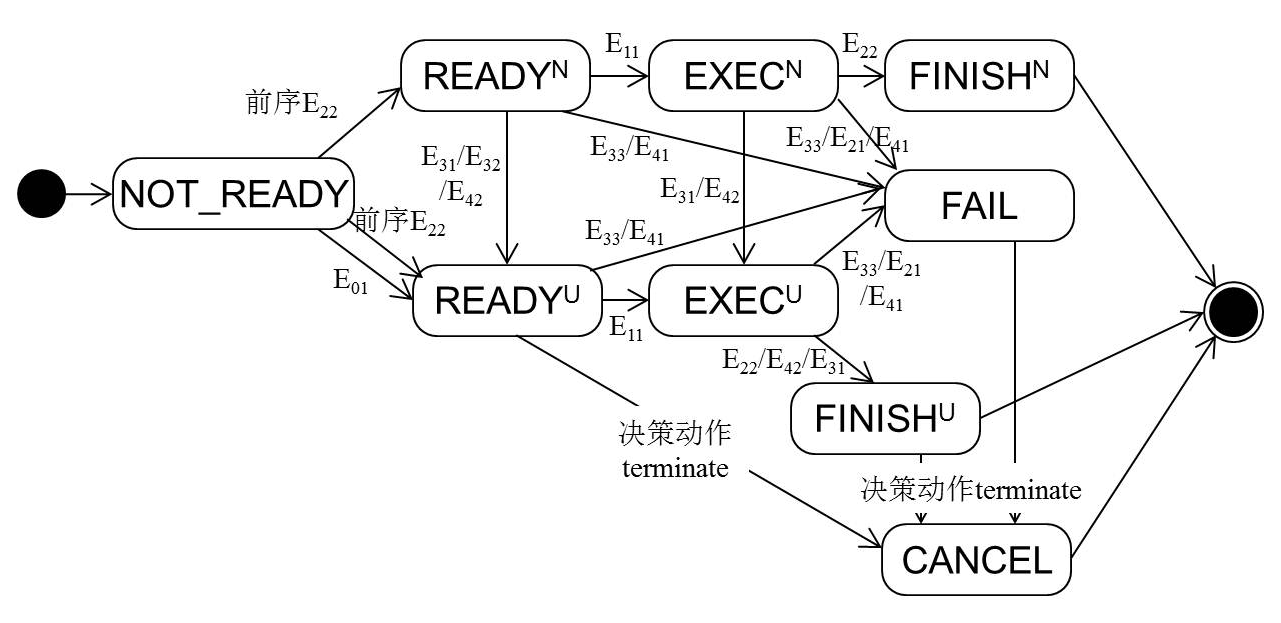
\includegraphics[width = 0.6\textwidth]{state_trans_bp}
%    \caption{业务层面服务活动的状态转换关系}\label{figure:state_trans_pb}
%    \vspace{-1em}
%\end{figure}
%
%业务层面服务活动之间的状态转换不同于如图~\ref{figure:state_trans}~所示的~Web Service~服务活动之间的状态转换,其不同点主要有:
%
%\begin{itemize}
%
%\item 业务服务在部分活动上即是~Web Service~,另一些活动是业务服务,因此具备业务层面不确定性;
%
%\item 业务层面在$READY$状态时会有用户的需求或者外部环境的变化,使得服务执行到另外的状态;而在纯的~Web Service~层面无需对$READY$状态的不确定性进行考虑;
%
%\item 业务层面在$EXEC$状态也会有用户的需求或者外部环境的变化而导致于服务执行状态发生变化,甚至于引起服务执行失败;而在~Web Service~层面仅仅需要等到服务执行完的事件触发~$E_{21}/E_{22}$~。
%
%\end{itemize}
%
%~b)~服务执行的整体状态
%
%在业务层面,由于不同的事件会使得流程执行到不同的状态,并且业务层面的需求和外部环境是可观察的,这与~Web Service~层面不同。因此,处理服务不确定性时需要确定是由用户需求导致的还是由外部环境变化导致的,从而整体服务流程的状态可由前锋线上的状态和不确定性事件源组合而成,如式(\ref{equation:state_total_bp})所示。
%
%\begin{equation}\label{equation:state_total_bp}
%state = < state(a_i),state(a_{i+1}),..., state(a_j), event >
%\end{equation}
%\begin{tabularx}{\textwidth}{@{}l@{\quad}l@{\pozhehao }X@{}}
%    式中
%    & $state(a_i)$ & 活动~$a_i$~的状态;\\
%    & $event$ & 使得服务处于当前状态的不确定性事件,如式(\ref{equation:event})所示。
%\end{tabularx}\vspace{\wordsep}
%
%业务层面的不确定性事件也包含软件层面的不确定性事件,而软件层面的不确定性事件是不可观测的,因此若服务状态是由软件层面的不确定性事件触发,则式(\ref{equation:state_total_bp})中的~$event$~取值为~$NULL$~,此时,按照软件层面的不确定性进行决策,如表~\ref{table:state_action}~所示。
%
%\paragraph{海运物流服务决策动作}
%
%业务层面的决策动作如同软件层面的决策动作,只是决策时刻不只是在服务执行结束时,而且在服务未执行时若有不确定性事件发生也会进行决策,换句话说,决策不仅包括对当前所执行服务的决策,并对预测的非正常服务也执行决策。
%
%同时,业务层面的不确定性一旦发生,就必须做出决策,这是因为无论用户需求发生变化还是外部环境发生变化,若不进行动作(不作为)则会导致业务执行下来不满足用户需求或者彻底失败,而这两种结果不是想要的结果。
%
%\paragraph{海运物流服务中事件、决策和状态之间的关系}
%
%要对业务层面的不确定性进行决策,需要知道业务层面导致于此类不确定性的原因(事件源),即是在如图~\ref{figure:state_trans_pb}~中体现出来即指向某状态的边上的事件,于是可以根据类似表~\ref{table:state_action}~中所示的软件层面不确定性而得出业务层面不确定性,如表~\ref{table:state_action_bp}~所示,此表与如图~\ref{figure:state_trans_pb}~中的事件和状态相一致。
%
%\begin{table}[htbp]
%    \caption{服务状态与决策动作之间的关系(业务层面)}
%    \vspace{-0.5em}\label{table:state_action_bp}\centering\zihao{5}
%    \begin{threeparttable}
%        \begin{tabular}{clclccc}
%            \toprule
%            事件源 & 状态类型\tnote{1} & 决策动作 & 决策后可能状态\tnote{1} & $r$~\tnote{2} & {$\Delta T$} & {$\Delta C$} \\
%            \midrule
%            
%            %------------------------------------------------------
%            {$E_{31}$} 
%            & {${READY^U}$}
%            & {终止}
%            & {$STOP$} 
%            & {0} 
%            & {0} 
%            & {$fc$} \\
%            
%            {}
%            & {}
%            & {替换} 
%            & {$FINISH$} 
%            & $R_{ik}\tnote{3}$ 
%            & {\multirow{2}{*}{$T_{ik}-T_{i0}$}} 
%            & {\multirow{2}{*}{$C_{ik}-C_{i0}$}} \\
%            
%            {}
%            & {}
%            & {} 
%            & {$FAIL$} 
%            & {0}
%            & {} 
%            & {} \\
%            
%            {}
%            & {}
%            & {重组} 
%            & {$FINISH^{N/U}$} 
%            & $R_{ik}\tnote{3}$ 
%            & {\multirow{2}{*}{$\sum\limits_{x = i}^j {({T_{xk}} - {T_{x0}})} $}}
%            & {\multirow{2}{*}{$\sum\limits_{x = i}^j {({C_{xk}} - {C_{x0}})} $}} \\
%            
%            
%            {}
%            & {}
%            & {} 
%            & {$FAIL$} 
%            & {0}
%            & {} 
%            & {} \\
%            
%            %------------------------------------------------------
%            {} 
%            & {${FAIL}$}
%            & {终止}
%            & {$STOP$} 
%            & {0} 
%            & {0} 
%            & {$fc$} \\
%            
%            {}
%            & \multicolumn{1}{r}{$/EXEC^U$}
%            & {替换} 
%            & {${FINISH}^{N/U}$} 
%            & $R_{ik}\tnote{3}$ 
%            & {\multirow{2}{*}{$T_{ik}$}} 
%            & {\multirow{2}{*}{$C_{ik}$}} \\
%            
%            {}
%            & {}
%            & {} 
%            & {$FAIL$} 
%            & {0}
%            & {} 
%            & {} \\
%            
%            {}
%            & {}
%            & {重组} 
%            & {$FINISH^{N/U}$} 
%            & $R_{ik}\tnote{3}$ 
%            & {\multirow{2}{*}{$T_{i0}+\sum\limits_{x = i}^j {({T_{xk}} - {T_{x0}})} $}}
%            & {\multirow{2}{*}{$C_{i0}+\sum\limits_{x = i}^j {({C_{xk}} - {C_{x0}})} $}} \\
%            
%            
%            {}
%            & {}
%            & {} 
%            & {$FAIL$} 
%            & {0}
%            & {} 
%            & {} \\
%            
%            %------------------------------------------------------
%            {} 
%            & {${FINISH^U}$}
%            & {终止}
%            & {$STOP$} 
%            & {0} 
%            & {0} 
%            & {$fc$} \\
%            
%            {}
%            & {}
%            & {重组} 
%            & {$FINISH^{N/U}$} 
%            & $R_{ik}\tnote{3}$ 
%            & {\multirow{2}{*}{$\sum\limits_{x = i}^j {({T_{xk}} - {T_{x0}})} $}}
%            & {\multirow{2}{*}{$\sum\limits_{x = i}^j {({C_{xk}} - {C_{x0}})} $}} \\
%            
%            
%            {}
%            & {}
%            & {} 
%            & {$FAIL$} 
%            & {0}
%            & {} 
%            & {} \\
%            %------------------------------------------------------
%            {$E_{32}$} 
%            & {$READY^U$}
%            & {替换} 
%            & {$FINISH$} 
%            & $R_{ik}\tnote{3}$ 
%            & {\multirow{2}{*}{$T_{ik}-T_{i0}$}} 
%            & {\multirow{2}{*}{$C_{ik}-C_{i0}$}} \\
%            
%            {}
%            & {}
%            & {} 
%            & {$FAIL$} 
%            & {0}
%            & {} 
%            & {} \\
%            
%            {}
%            & {}
%            & {重组} 
%            & {$FINISH^{N/U}$} 
%            & $R_{ik}\tnote{3}$ 
%            & {\multirow{2}{*}{$\sum\limits_{x = i}^j {({T_{xk}} - {T_{x0}})} $}}
%            & {\multirow{2}{*}{$\sum\limits_{x = i}^j {({C_{xk}} - {C_{x0}})} $}} \\
%            
%            
%            {}
%            & {}
%            & {} 
%            & {$FAIL$} 
%            & {0}
%            & {} 
%            & {} \\
%            
%            %------------------------------------------------------
%            {$E_{33}$} 
%            & {${READY^U}$}
%            & {终止}
%            & {$STOP$} 
%            & {0} 
%            & {0} 
%            & {$fc$} \\
%            %------------------------------------------------------
%            {$E_{41}$} 
%            & {${FAIL^U}$}
%            & {终止}
%            & {$STOP$} 
%            & {0} 
%            & {0} 
%            & {$fc$} \\
%            
%            {}
%            & {}
%            & {替换} 
%            & {$FINISH$} 
%            & $R_{ik}\tnote{3}$ 
%            & {\multirow{2}{*}{$T_{ik}$}} 
%            & {\multirow{2}{*}{$C_{ik}$}} \\
%            
%            {}
%            & {}
%            & {} 
%            & {$FAIL$} 
%            & {0}
%            & {} 
%            & {} \\
%            
%            {}
%            & {}
%            & {重组} 
%            & {$FINISH^{N/U}$} 
%            & $R_{ik}\tnote{3}$ 
%            & {\multirow{2}{*}{$T_{i0}+\sum\limits_{x = i}^j {({T_{xk}} - {T_{x0}})} $}}
%            & {\multirow{2}{*}{$C_{i0}+\sum\limits_{x = i}^j {({C_{xk}} - {C_{x0}})} $}} \\
%            
%            
%            {}
%            & {}
%            & {} 
%            & {$FAIL$} 
%            & {0}
%            & {} 
%            & {} \\
%            %------------------------------------------------------
%            {$E_{42}$} 
%            & {${READY^U}$}
%            & {终止}
%            & {$STOP$} 
%            & {0} 
%            & {0} 
%            & {$fc$} \\
%            
%            {}
%            & {}
%            & {替换} 
%            & {$FINISH$} 
%            & $R_{ik}\tnote{3}$ 
%            & {\multirow{2}{*}{$T_{ik}-T_{i0}$}} 
%            & {\multirow{2}{*}{$C_{ik}-C_{i0}$}} \\
%            
%            {}
%            & {}
%            & {} 
%            & {$FAIL$} 
%            & {0}
%            & {} 
%            & {} \\
%            
%            {}
%            & {}
%            & {重组} 
%            & {$FINISH^{N/U}$} 
%            & $R_{ik}\tnote{3}$ 
%            & {\multirow{2}{*}{$\sum\limits_{x = i}^j {({T_{xk}} - {T_{x0}})} $}}
%            & {\multirow{2}{*}{$\sum\limits_{x = i}^j {({C_{xk}} - {C_{x0}})} $}} \\
%            
%            
%            {}
%            & {}
%            & {} 
%            & {$FAIL$} 
%            & {0}
%            & {} 
%            & {} \\
%            %------------------------------------------------------
%            {} 
%            & {${EXEC^U}$}
%            & {终止}
%            & {$STOP$} 
%            & {0} 
%            & {0} 
%            & {$fc$} \\
%            
%            {}
%            & \multicolumn{1}{r}{$/FINISH^U$}
%            & {替换} 
%            & {$FINISH$} 
%            & $R_{ik}\tnote{3}$ 
%            & {\multirow{2}{*}{$T_{ik}$}} 
%            & {\multirow{2}{*}{$C_{ik}$}} \\
%            
%            {}
%            & {}
%            & {} 
%            & {$FAIL$} 
%            & {0}
%            & {} 
%            & {} \\
%            
%            {}
%            & {}
%            & {重组} 
%            & {$FINISH^{N/U}$} 
%            & $R_{ik}\tnote{3}$ 
%            & {\multirow{2}{*}{$T_{i0}+\sum\limits_{x = i}^j {({T_{xk}} - {T_{x0}})} $}}
%            & {\multirow{2}{*}{$C_{i0}+\sum\limits_{x = i}^j {({C_{xk}} - {C_{x0}})} $}} \\
%            
%            
%            {}
%            & {}
%            & {} 
%            & {$FAIL$} 
%            & {0}
%            & {} 
%            & {} \\
%            
%            \bottomrule
%        \end{tabular}%
%        
%        \begin{tablenotes}
%            \item[1] 决策动作前状态所带参数为$(T,C)$, 决策后状态参数变为~$(T+\Delta T, C+\Delta C)$,~ 其中~$\Delta T \ge 0$, ~$\Delta C \ge 0$~; 
%            \item[2] $r$~为决策后,服务可继续执行的概率;
%            \item[3] $S_{ik}$~为替换后的服务或者重组后最先执行的服务,~$R_{ik}$~为此服务的可靠性。
%        \end{tablenotes}
%    \end{threeparttable}
%\end{table}%
%
%\paragraph{海运物流服务决策收益}
%
%决策收益的计算方式与软件层面的决策收益一致,其中~$r$~、~$\Delta T$~、 ~$\Delta C$~的计算方式如表~\ref{table:state_action_bp}~右侧的三列所示。
%
%%\paragraph{不确定性触发关系图}
%%
%%业务层面不确定性触发关系图同~\ref{sec:utg}~介绍一样。
%
%\paragraph{海运物流业务的不确定性决策系统}
%
%在海运物流中,如图~\ref{figure:bp_example}~所示的业务流程,可针对每个可~IT~化的活动,开发出支持此活动的~Web Service~(例如图~\ref{figure:bp_example}~所示的活动~$a_{4}$~:预订舱位),而其余只能人工作的活动(例如图~\ref{figure:bp_example}~所示的活动~$a_{14}$~:装箱)则无需开发。
%
%开发软件层面的原型系统之后,针对海运物流的具体业务流程,开发针对海运物流的不确定性决策系统,其底层由软件层面的原型系统提供支持,上层运行海运物流的业务流程。其系统结构如图~\ref{figure:app_system}~所示。
%
%\begin{figure}[htbp]
%    \centering
%    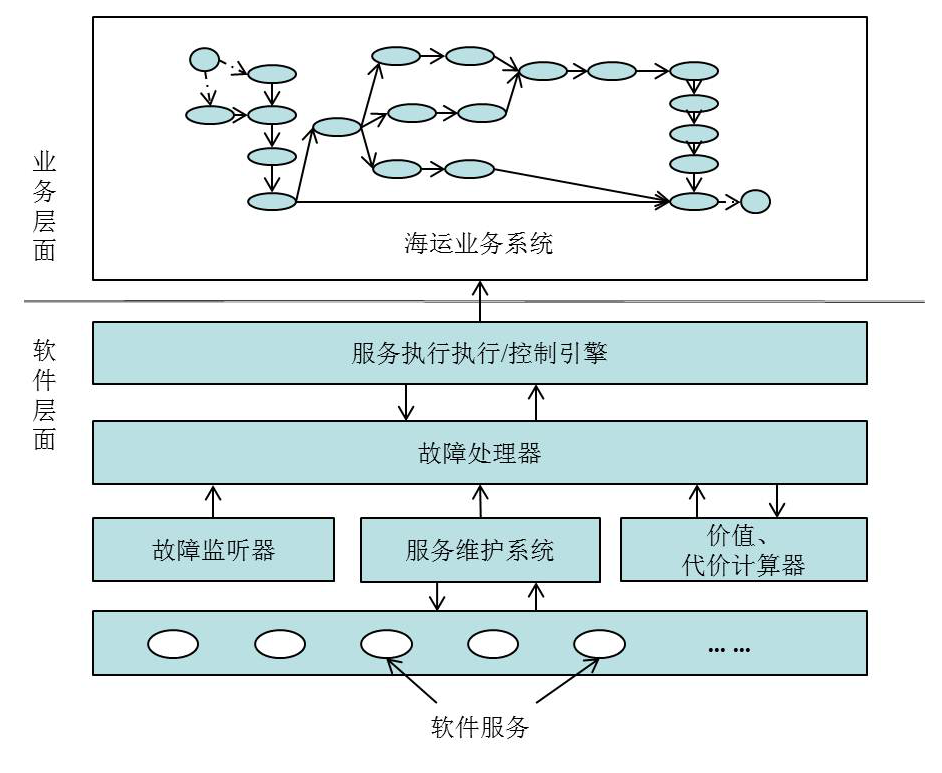
\includegraphics[width = 0.7\textwidth]{app_system}
%    \caption{支持不确定性决策的海运物流业务系统结构}\label{figure:app_system}
%    \vspace{-1em}
%\end{figure}

%-------------------------------------------

